\documentclass[12pt,a4paper]{report}

% ===== PACKAGES =====
\usepackage[utf8]{inputenc}
\usepackage{geometry}
\usepackage{setspace}
\usepackage{titlesec}
\usepackage{fancyhdr}
\usepackage{graphicx}
\usepackage{tocloft}
\usepackage[numbers]{natbib}
\usepackage{amsmath}
\usepackage{amssymb}
\usepackage{booktabs}
\usepackage{longtable}
\usepackage{array}
\usepackage{chngcntr}
\usepackage{microtype}   % smoother line-breaking, fewer overfull-hbox overruns
\usepackage{ragged2e}    % \RaggedRight for cells that must not overflow
\usepackage{tabularx}
\usepackage{float}      % [H] float specifier: forces tables/figures to stay exactly
                         % where placed in the source, instead of drifting elsewhere
\usepackage{framed}     % boxed code/prompt exhibits containing a verbatim block --
                         % fbox cannot wrap a verbatim environment (its brace-delimited
                         % argument is grabbed before verbatim's catcodes take effect, so
                         % the raw braces inside the verbatim text desync the brace count);
                         % the framed environment is a true environment, not a macro
                         % argument, so it does not have this problem
\usepackage{makecell}    % \makecell for two-line table headers, so a long metric-name
                         % header does not force its column wider than its (short,
                         % numeric) data actually needs
\usepackage{changepage}  % adjustwidth: narrows content width like minipage, but (unlike
                          % minipage) still allows a page break inside -- needed so a tall
                          % framed/verbatim block can flow across pages instead of being
                          % forced onto one page and overflowing past the bottom margin

\usepackage{seqsplit}
\usepackage{multirow}
\usepackage{adjustbox}

                          % ===== PAGE SETUP =====
\geometry{margin=1in}
\setstretch{1.5}
\setlength{\headheight}{14pt}
\emergencystretch=2em    % lets LaTeX stretch a line slightly instead of spilling into the margin
\sloppy                  % prefer looser spacing over text running past the right margin

% Number tables/figures per chapter (e.g., Table 4.1, Figure 3.1)
\counterwithin{table}{chapter}
\counterwithin{figure}{chapter}

% ===== HEADER FOOTER =====
\pagestyle{fancy}
\fancyhf{}
\fancyhead[R]{FPT School of Business \& Technology}
\fancyfoot[R]{Do Minh Hieu - MSE13172}
\fancyfoot[C]{\thepage}
\renewcommand{\headrulewidth}{0.4pt}
\renewcommand{\footrulewidth}{0.4pt}
% Chapter-opening and front-matter pages use the "plain" style; give them the same header/footer
\fancypagestyle{plain}{%
    \fancyhf{}%
    \fancyhead[R]{FPT School of Business \& Technology}%
    \fancyfoot[R]{Do Minh Hieu - MSE13172}%
    \fancyfoot[C]{\thepage}%
}
% Longtable captions span the full text width like the other tables
\setlength{\LTcapwidth}{\textwidth}
% Let large floats sit at the top of a page with text below, instead of on a
% half-empty float page; any float page that remains starts at the top
\renewcommand{\topfraction}{0.9}
\renewcommand{\bottomfraction}{0.8}
\renewcommand{\textfraction}{0.07}
\renewcommand{\floatpagefraction}{0.9}
\makeatletter
\setlength{\@fptop}{0pt}
\makeatother

% ===== TOC STYLE (đẹp hơn mặc định) =====
\renewcommand{\cftchapfont}{\bfseries}
\renewcommand{\cftchappagefont}{\bfseries}

% Keep the bibliography heading as "References" (report class defaults to "Bibliography")
\renewcommand{\bibname}{References}
\newcommand{\myfig}[3]{%
    \begin{figure}[H]
        \centering
        \adjustbox{max width=0.85\textwidth, max height=0.75\textheight, center}{%
            \includegraphics{#1}%
        }
        \caption{#2}
        \label{#3}
    \end{figure}
}
% ===== HYPERLINKS (must load after tocloft/natbib/most other packages) =====
% Makes the Table of Contents, List of Tables, List of Figures, and \ref/\cite
% entries actual clickable links that jump to the right page/figure/table/citation,
% and adds PDF bookmarks for navigation.
\PassOptionsToPackage{hyphens}{url} % allow long reference URLs to break at hyphens
\usepackage[colorlinks=true, linkcolor=blue, citecolor=blue, urlcolor=blue, bookmarksnumbered=true]{hyperref}

\begin{document}

% ===================== COVER PAGE =====================
\begin{titlepage}
    \centering

    \vspace*{0.5cm}

    % Logo
    \includegraphics[width=0.4\textwidth]{src-v2/figures/2025-LOGO-FSB.png}

    \vspace{1.5cm}

    {\large \textbf{MASTER'S THESIS}}

    \vspace{1.5cm}

    \rule{0.85\textwidth}{0.5pt}

    \vspace{1cm}

    {\large \textbf{
    SEMANTIC LANE AND TRAFFIC SIGN UNDERSTANDING USING VISION-LANGUAGE MODELS FOR DRIVING DECISION SUPPORT
    }}

    \vspace{0.5cm}

    % NOTE(author): plain pdfLaTeX + inputenc/utf8 cannot render Vietnamese diacritics
    % (o-horn, u-horn, tone marks). Compile with XeLaTeX/LuaLaTeX + fontspec and a
    % Unicode font to enable the line below; left commented out to keep pdfLaTeX builds
    % working out of the box.
    % {\normalsize \textit{(Vietnamese title: Hiểu Làn đường và Biển báo Giao thông
    % theo Ngữ nghĩa sử dụng Mô hình Thị giác - Ngôn ngữ để Hỗ trợ Ra quyết định Lái xe)}}

    \vspace{1cm}

    \rule{0.85\textwidth}{0.5pt}

    \vspace{2cm}

    \begin{tabular}{rl}
        \textbf{Academic Supervisor:} & Dr. Doan Nhat Quang \\
        \textbf{Student:} & Do Minh Hieu - MSE13172\\
    \end{tabular}

    \vfill

    {\normalsize Hanoi, 2026}

\end{titlepage}
% ===================== FRONT MATTER =====================
% Front matter (Declaration ... List of Abbreviations) uses its own roman-numeral
% page sequence (i, ii, iii, ...), separate from the arabic sequence that Chapter 1
% restarts below -- otherwise both sequences default to arabic and collide/overlap
% in the Table of Contents (e.g., Chapter 1 appearing at a lower page number than
% List of Abbreviations).
\pagenumbering{roman}
\clearpage

\chapter*{Declaration}
\phantomsection
\addcontentsline{toc}{chapter}{Declaration}
I, \textbf{Do Minh Hieu}, student ID \textbf{MSE13172}, hereby declare that this thesis, entitled \textit{Semantic Lane and Traffic Sign Understanding Using Vision-Language Models for Driving Decision Support}, is my own work, carried out under the academic supervision of Dr. \textbf{Doan Nhat Quang}.

The data and experimental results presented in this thesis are truthful, collected and processed using tools and source code that I built myself, and have not been published in any other work. Content referenced from the work of other authors is fully and clearly cited in the References section.

Should any dishonesty or violation of scientific integrity regulations be found, I take full responsibility before the Thesis Committee and the University.

\chapter*{Acknowledgments}
\phantomsection
\addcontentsline{toc}{chapter}{Acknowledgments}
To complete this Master's program and this research, beyond my own effort, I have received enormous teaching, guidance, and encouragement from my teachers, my university, my friends, and my family.

First, I would like to express my sincere gratitude to my thesis supervisor, Dr. \textbf{Doan Nhat Quang}. He is the one who inspired and guided me in shaping the idea for this research topic, and who spent a great deal of time instructing me, sharing knowledge, and reviewing and commenting throughout the course of this work. His dedicated guidance not only helped me complete this thesis but will also be valuable groundwork for my professional development going forward.

I sincerely thank the faculty and staff at the \textbf{FPT School of Business \& Technology (FSB)} for creating a professional, open educational environment in which I could build a solid foundation of specialized knowledge and take part in valuable seminars. I would also like to thank my friends and colleagues, who were always willing to share knowledge, discuss ideas, and accompany me throughout my studies.

Finally, I would like to devote my deepest affection and boundless gratitude to my parents and siblings. My family has always been my firmest anchor, providing peace of mind, trust, and the best possible conditions for me to persevere through difficulties and complete my academic dream.

Despite considerable effort in carrying out and presenting this research, certain limitations remain unavoidable. I sincerely welcome any valuable feedback from the members of the Thesis Committee so that this work can be further improved.

\clearpage
\tableofcontents

\clearpage
\phantomsection
\addcontentsline{toc}{chapter}{List of Tables}
\listoftables

\clearpage
\phantomsection
\addcontentsline{toc}{chapter}{List of Figures}
\listoffigures

\clearpage
\chapter*{List of Abbreviations}
\phantomsection
\addcontentsline{toc}{chapter}{List of Abbreviations}
\begin{longtable}{
    >{\RaggedRight\arraybackslash}p{2.7cm}
    >{\RaggedRight\arraybackslash}p{4.2cm}
    >{\RaggedRight\arraybackslash}p{7.0cm}
}
    \caption*{List of abbreviations.}
    \label{tab:abbreviations} \\
    \toprule
    \textbf{Abbreviation} & \textbf{English} & \textbf{Explanation} \\
    \midrule
    \endfirsthead
    \caption*{List of abbreviations. (continued)} \\
    \toprule
    \textbf{Abbreviation} & \textbf{English} & \textbf{Explanation} \\
    \midrule
    \endhead
    \midrule
    \multicolumn{3}{r}{\footnotesize\itshape Continued on next page\ldots} \\
    \endfoot
    \bottomrule
    \endlastfoot
    ADAS & Advanced Driver Assistance System & An advanced driver assistance system \\
    API & Application Programming Interface & An application programming interface \\
    BDD100K & Berkeley DeepDrive 100K & A large-scale multi-task driving dataset \\
    BEV & Bird's-Eye View & A top-down spatial representation \\
    CIoU & Complete Intersection over Union & An IoU-based box-regression loss that also accounts for center distance and aspect ratio \\
    CNN & Convolutional Neural Network & A convolutional neural network \\
    COCO & Common Objects in Context & A general-purpose object-detection dataset \\
    CPU & Central Processing Unit & A central processing unit \\
    CUDA & Compute Unified Device Architecture & NVIDIA's parallel computing platform for GPUs \\
    DFL & Distribution Focal Loss & A distribution-based loss for box-boundary regression \\
    F1 & F1-score & The harmonic mean of Precision and Recall \\
    FLTTA & Feature-Level Test-Time Augmentation & Test-time augmentation applied by shifting backbone features \\
    FPN & Feature Pyramid Network & A feature pyramid network \\
    FPS & Frames Per Second & The number of frames processed per second \\
    GFLOPs & Giga Floating-Point Operations & Billions of floating-point operations \\
    GPU & Graphics Processing Unit & A graphics processing unit \\
    GTSRB & German Traffic Sign Recognition Benchmark & A German traffic-sign classification dataset \\
    IoU & Intersection over Union & A localization metric \\
    JSON & JavaScript Object Notation & The structured data format used to realize SSI \\
    LiDAR & Light Detection and Ranging & A laser-based range sensor \\
    LISA & Laboratory for Intelligent and Safe Automobiles & A traffic-sign dataset from the LISA laboratory \\
    LLM & Large Language Model & A large language model \\
    LSTM & Long Short-Term Memory & A long short-term memory network \\
    MAE & Mean Absolute Error & Mean absolute error \\
    mAP & mean Average Precision & The average precision averaged over classes \\
    MLLM & Multimodal Large Language Model & A multimodal large language model \\
    MLP & Multi-Layer Perceptron & A multi-layer perceptron \\
    MSE & Mean Squared Error & Mean squared error \\
    NIM & NVIDIA Inference Microservices & NVIDIA's model-inference service (the platform used to call the VLM in this thesis) \\
    NMS & Non-Maximum Suppression & Removal of duplicate predicted boxes \\
    RAG & Retrieval-Augmented Generation & Text generation augmented with retrieval \\
    RGB & Red--Green--Blue & A three-channel color image (red, green, blue) \\
    RT-DETR & Real-Time Detection Transformer & A transformer-based real-time object detector \\
    SGD & Stochastic Gradient Descent & The stochastic gradient descent optimization algorithm \\
    SSI & Structured Semantic Information & Structured semantic information, $\mathrm{SSI}=\Phi(L,T)$, derived from the lane- and traffic-sign-detection outputs \\
    TT100K & Tsinghua-Tencent 100K & A large-scale traffic-sign dataset \\
    UFLD-v2 & Ultra Fast Lane Detection v2 & A high-speed lane-detection architecture (version 2) \\
    VLM & Vision-Language Model & A vision-language model \\
    YOLO & You Only Look Once & A family of single-stage object-detection architectures \\
\end{longtable}

% ===================== MAIN CONTENT =====================
\clearpage
\pagenumbering{arabic}
\setcounter{page}{1}

\chapter{Introduction}

\section{Background and Motivation}

Advanced Driver Assistance Systems (ADAS) are a class of electronic systems that use sensors such as cameras, radar, and LiDAR to perceive the traffic environment and support the driver in tasks such as lane-departure warning, lane-keeping assistance, and automatic emergency braking \cite{nidamanuri2022adas}. The development of these systems has important implications for traffic safety, against a backdrop in which road accidents cause roughly 1.19 million deaths per year worldwide \cite{who2023roadsafety}. Several driver-assistance functions based on lane perception have been shown to substantially reduce the risk of collisions and related injuries \cite{iihs2017lanedeparture}.

Vision-language models (VLMs) open up a new approach to driver assistance. A VLM can take in an image together with natural language to describe, reason about, or explain a traffic situation \cite{xu2024drivegpt4,rivera2025scenario}, and can thereby synthesize multiple observations into a situation assessment and a driving recommendation in natural language.

However, requiring a VLM to carry out all of the reasoning directly from an RGB image also raises challenges. Quantitative spatial relationships, such as the vehicle's position relative to the lane or the geometry of the lane markings, can be difficult for the model to exploit consistently from the image \cite{tong2024eyeswideshut,kamath2023whatsup}. At the same time, a generative model can produce information that has no observable evidence, leading to hallucination \cite{ji2023hallucination,li2023pope}. In traffic applications, these limitations are particularly concerning because recommendation quality depends on the ability to correctly use the evidence relevant to the situation.

One approach to mitigating these limitations is to supply the model with additional information in the form of a structured representation. Retrieval-Augmented Generation (RAG) allows a model to use structured external information to support the generation process \cite{lewis2020rag}; in the driving domain, DriveVLM \cite{tian2024drivevlm} and Talk2BEV \cite{choudhary2024talk2bev} also show that combining a VLM with structured spatial or semantic representations can support the reasoning process. These works are analyzed in detail in Chapter 2.

From this, the question arises whether structured semantic information extracted from specialized detection models actually creates added value for a VLM in generating driving recommendations. This is the main motivation of the thesis.

\section{Research Gap and Problem Statement}

In computer-vision-based ADAS, the traffic environment is typically perceived through specialized modules such as lane detection, traffic sign detection, and vehicle detection. The outputs of these models are usually low-level representations such as pixel coordinates, bounding boxes, class IDs, or geometric points of the lanes. These representations are suitable for recognition tasks but do not express the traffic situation in the kind of semantics that a person can use to make a decision.

For example, a lane-detection model can identify the points belonging to two lane markings, while a traffic sign detection model returns a bounding box and a class ID. The information useful to the driver, however, is: which lane the vehicle is in, how far it is offset from the lane center, whether the road is straight or curved, and which traffic signs are present. This gap creates the need for an intermediate processing layer that converts detection results into structured, easily interpretable traffic information.

From the review in Chapter 2, this thesis identifies that the role of semantic information built directly from the outputs of lane- and traffic-sign-detection models in the quality of VLM driving recommendations has not been clarified in the work within the scope of the survey. Therefore, the research problem is stated as follows: build a process that converts the outputs of lane- and traffic-sign-detection models into Structured Semantic Information (SSI), and then use SSI as a source of context for a VLM when analyzing the situation and generating driving recommendations in natural language. The role of SSI is evaluated through a controlled comparative experiment on the same VLM and the same dataset.

\section{Research Objectives}

Based on the analysis in Section 1.2, this thesis focuses on three problems: building SSI from lane- and traffic-sign-detection results, integrating SSI into a VLM to support recommendation generation, and quantitatively evaluating the role of SSI in recommendation quality.

The main objectives are:

\textbf{Understanding traffic semantics:} Build a module that extracts and organizes information from lane- and traffic-sign-detection results into SSI.

\textbf{Generating driving recommendations based on SSI:} Build a method for supplying SSI to the VLM together with the input image, thereby supporting the VLM in analyzing the traffic situation and generating driving recommendations in natural language.

\textbf{Evaluating the role of SSI in recommendation generation:} Quantify the change in recommendation quality when SSI is added, compared with the condition in which only the input image is used.

\section{Research Contributions}

Based on the objectives in Section 1.3, this thesis focuses on two main contributions:

\textbf{This thesis develops a pipeline for traffic semantic analysis and driving-recommendation generation.} The pipeline consists of two modules: (i) extracting SSI from the lane- and traffic-sign-detection results using geometric and deterministic rules, without any additional machine-learning model or learnable parameters; and (ii) supplying SSI together with the input image to the VLM through a prompt, with rules for using and resolving conflicts between the pieces of evidence, to support situation analysis and the generation of driving recommendations in natural language without fine-tuning the VLM.

\textbf{This thesis proposes a controlled evaluation framework for the role of SSI.} The framework compares input modes with and without SSI on the same VLM and the same data, scores the recommendations with a six-criterion rubric, and uses multiple LLM-as-a-Judge models together with paired statistical tests; conclusions are drawn from trends that are consistent across the judges rather than from the absolute scores of any single judge. In this way, it quantifies the change in recommendation quality when SSI is added and analyzes how this change varies with the accuracy of SSI.

\section{Thesis Structure}

The thesis consists of five chapters:

\textbf{Chapter 1 -- Introduction:} background and motivation, the research gap, the problem statement, and the objectives and contributions of the thesis.

\textbf{Chapter 2 -- Literature Review and Theoretical Background:} lane and traffic sign detection methods, directions for applying VLM/LLM to traffic, and the LLM-as-a-Judge evaluation method; from these, the gap addressed by the thesis is identified.

\textbf{Chapter 3 -- Proposed Methodology:} the problem formulation and assumptions, the pipeline architecture, the basis for selecting models and data, the SSI extraction algorithms, the prompt design for the three input modes, and the evaluation method (rubric, scoring protocol, statistical testing).

\textbf{Chapter 4 -- Experiments and Results:} the experimental setup; evaluation of the SSI extraction module and of SSI quality on CULane and on the self-collected data; VLM selection; the controlled experiment across the three input modes; comparison of the judges with human evaluation; and two supplementary experiments on the VLM's ability to self-extract SSI and on the influence of the prompt.

\textbf{Chapter 5 -- Conclusion and Future Work:} a summary of the contributions, a discussion of the limitations, and proposed directions for further research.

\chapter{Literature Review and Theoretical Background}

Advanced Driver Assistance Systems (ADAS) have become common equipment on commercial vehicles, with functions such as lane-departure warning, lane-keeping assistance, and traffic sign detection. Nidamanuri et al. \cite{nidamanuri2022adas} show that ADAS is shifting from systems based on a single sensor toward multi-sensor systems combined with deep learning, in order to increase reliability under diverse real-world conditions. Beyond perception accuracy, the need to explain the system's decisions to the driver opens a role for models capable of generating natural language. This chapter reviews related research along three topics, corresponding to the components of the proposed pipeline: lane and traffic sign detection (Section 2.1), applications of VLM/LLM in traffic (Section 2.2), and the LLM-as-a-Judge evaluation method (Section 2.3).

\section{Lane and Traffic Sign Detection}

\subsection{Lane Detection}

Lane detection is the task of locating lane markings or lane boundaries in an image, serving as the basis for the lane-departure warning and lane-keeping assistance features of ADAS. Among deep-learning methods, three common approaches are \cite{zhang2021survey,zakaria2023slr}: (a) semantic segmentation, which identifies the pixels that belong to a lane; (b) row/column classification, which predicts the lane position at discrete image rows or columns; and (c) anchor-based mechanisms, which use candidate lines as the basis for predicting and refining lanes. These approaches involve different trade-offs between geometric accuracy and inference speed.

In the row/column classification approach, Ultra Fast Lane Detection (UFLD) and UFLD-v2 \cite{qin2022ufldv2} focus on inference speed by turning lane detection into a problem of classifying positions over image rows/columns. In the anchor-based approach, LaneATT \cite{tabelini2021laneatt} uses an attention mechanism over line anchors, while CLRNet \cite{zheng2022clrnet} refines lanes across multiple feature levels and uses Line IoU to optimize geometric fit. These models represent different choices in how lane geometry is represented and processed.

For the problem of this thesis, the requirement for the lane-detection model is not only accuracy but also the form of the output: the model must provide point coordinates on each boundary to support the geometric computations in the next step. This criterion, together with the deployment constraints, is the basis for model selection in Section 3.3.2. Because UFLD-v2 is the model used, its architecture is presented below (Figure~\ref{fig:ufldv2}).

\begin{figure}[H]
    \centering
    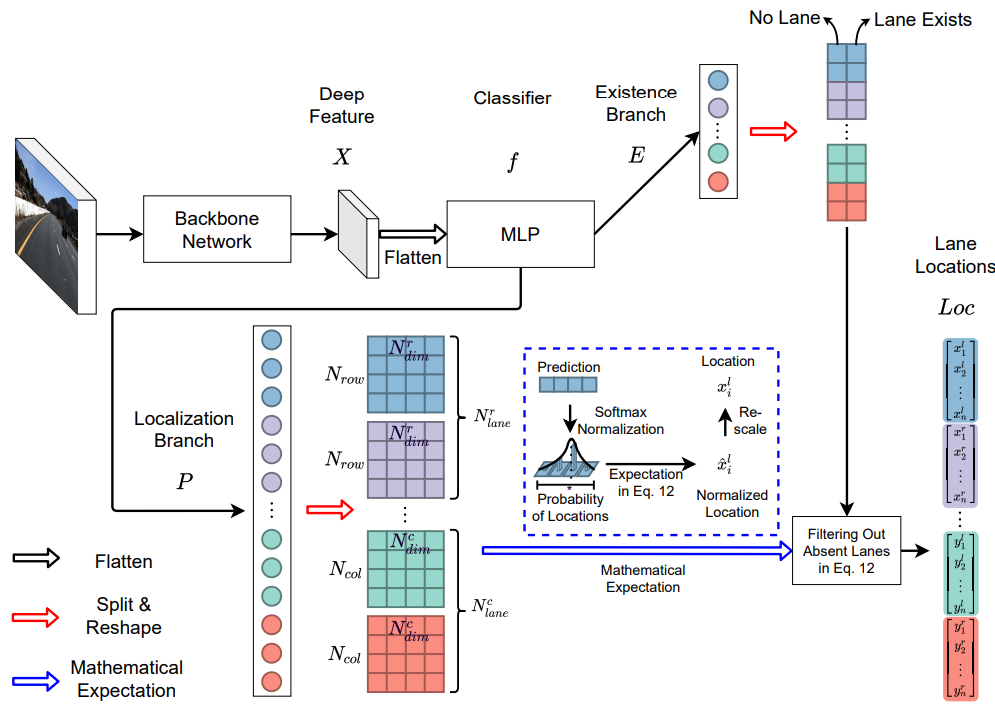
\includegraphics[
        width=0.75\textwidth,
        height=0.65\textheight,
        keepaspectratio
    ]{src-v2/figures/ufldv2.png}
    \caption[Overall architecture of UFLD-v2.]{Overall architecture of UFLD-v2 (source: \cite{qin2022ufldv2}).}
    \label{fig:ufldv2}
\end{figure}

The Backbone Network extracts deep features $X$ from the input image, which are passed through a classifier (MLP) $f$ to produce two parallel prediction branches: the Existence Branch $E$ predicts whether each lane boundary exists; the Localization Branch $P$ predicts position over a row/column grid ($N_{row}$/$N_{col}$). The positional probability distribution is used to compute the expected value, from which a continuous coordinate (Loc) is derived. Boundaries predicted as non-existent are removed from the final output. The set of point coordinates on these lane boundaries is used as the input to the SSI extraction module of this thesis (Section 3.4.1).

\subsection{Traffic Sign Detection}

Traffic sign detection is the task of localizing and classifying traffic signs in an image. Two common approaches are two-stage detectors (proposing candidate regions and then classifying them, e.g., Mask R-CNN) and single-stage detectors (predicting location and class in a single inference pass, e.g., the YOLO family). The difficulty of the task depends on the number of target classes and on the size of the signs in the image: distant signs often occupy only a very small region. Unlike classification on already-cropped images, detection is subject to both localization errors and classification errors.

YOLOv8 \cite{sapkota2025yoloevolution} is a single-stage detector in the YOLO family \cite{redmon2016yolo}, used in many traffic sign detection studies because of its balance between speed and accuracy. Because YOLOv8 is the model used for the traffic sign detection step (Section 3.3.3), its architecture is summarized below (Figure~\ref{fig:yolov8}).

\begin{figure}[H]
    \centering
    \includegraphics[
        width=0.75\textwidth,
        height=0.65\textheight,
        keepaspectratio
    ]{src-v2/figures/yolov8_architecture_diagram.png}
    \caption[Schematic overview of the YOLOv8 architecture.]{Schematic overview of the YOLOv8 architecture (source: \cite{sapkota2025yoloevolution}).}
    \label{fig:yolov8}
\end{figure}

The YOLOv8 architecture consists of four components:

\begin{itemize}
    \item \textbf{Backbone:} extracts feature maps C1--C5 with decreasing resolution and increasing semantic level; the three deepest stages, C3, C4, and C5, are passed to the FPN. The backbone and neck use lightweight C2f blocks \cite{sapkota2025yoloevolution}.
    \item \textbf{FPN (Feature Pyramid Network):} combines multi-scale features in a top-down flow. Features at a deeper level are upsampled $\times2$ and concatenated with the backbone features at the next level (C4, then C3), so that the high-resolution feature maps are enriched with semantic information.
    \item \textbf{Feature Pyramid and Head:} the FPN produces three feature maps, P3, P4, and P5, corresponding to three object scales, and each level has its own Head. The Head is \textit{decoupled} into a classification branch and a box-regression branch, and is \textit{anchor-free} \cite{sapkota2025yoloevolution}.
    \item \textbf{Loss function:} Figure~\ref{fig:yolov8} depicts the loss block in the general form used in \cite{sapkota2025yoloevolution}; in the Ultralytics implementation of YOLOv8 used in this thesis, box regression uses the CIoU loss combined with Distribution Focal Loss (DFL), and classification uses a classification loss over $K$ classes \cite{jocher2023yolov8}.
\end{itemize}

At inference time, the predictions from the three levels are merged and filtered by Non-Maximum Suppression (NMS). The n/s/m/l/x variants differ only in the depth and width multipliers of the network (Table~\ref{tab:3.5}). For traffic signs, the P3 level matters most because distant signs often occupy only a few dozen pixels; this is also the focus of the improvements in \cite{ji2024improvedyolov8}.

Tabernik and Sko{\v c}aj \cite{tabernik2020largescale} use Mask R-CNN to detect and classify a large number of sign types, showing the scalability of two-stage detectors. Recent work integrates attention/transformer mechanisms into YOLOv8 to improve small-object detection: Logeswaran et al. \cite{logeswaran2024pedestrian} detect pedestrians and traffic signs simultaneously; Ji et al. \cite{ji2024improvedyolov8} add BoTNet, ODConv, and LSKA to YOLOv8n on TT100K.

The studies above focus on improving the ability to detect and classify traffic signs. In this thesis, the traffic sign detection result is not the final output but the input to the semantic representation step, where the class and position of the signs are organized into structured attributes to be supplied to the VLM.

\section{Vision-Language Models (VLMs) for Traffic Applications}

A vision-language model (VLM) is a multimodal model that extends a text-only LLM to accept both images and text, typically with three components: a visual encoder that extracts image features, a projection layer that maps the visual features into the LLM's embedding space, and the LLM that generates text. There are two ways to exploit a VLM: fine-tuning on specialized data, or using a general-purpose VLM as-is (training-free) through prompt design. The second approach has lower deployment cost but depends more heavily on the quality of the context and prompt. This thesis follows the second approach: the VLM is used through an API as a black-box model, so its architecture is presented only at a general level.

The idea of encoding traffic semantics into a structured representation to support behavioral reasoning appeared before the LLM era. Hong et al. \cite{hong2019rules} encode the high-level semantics of a traffic situation into a spatial grid so that a deep-learning model can predict driving behavior. However, this work does not aim at generating recommendations or explanations in natural language. With the emergence of LLMs/VLMs, recent work can be grouped into three categories according to the role of the language model in the pipeline (Table~\ref{tab:2.1}).

\begin{table}[!htbp]
    \centering
    \setstretch{1.5}
    \footnotesize
    \renewcommand{\arraystretch}{1.25}
    \caption{Summary of related work on LLM/VLM for driving.}
    \label{tab:2.1}
    \begin{tabularx}{\linewidth}{
        >{\RaggedRight\arraybackslash}p{3.0cm}
        >{\RaggedRight\arraybackslash}p{3.6cm}
        >{\RaggedRight\arraybackslash}X
    }
        \toprule
        \textbf{Group} & \textbf{Work} & \textbf{Main technical characteristics} \\
        \midrule
        Large-scale end-to-end & DriveGPT4 \cite{xu2024drivegpt4} & Generates natural-language explanations together with control signals, trained end-to-end \\
         & DriveLM \cite{sima2024drivelm} & Frames driving as Graph Visual Question Answering \\
         & LMDrive \cite{shao2024lmdrive} & Closed-loop end-to-end driving with an LLM \\
        Added interaction/ reasoning layer & Drive as You Speak \cite{cui2024driveasyouspeak} & LLM tool use, reasoning and acting, personalized interaction \\
         & DriveVLM \cite{tian2024drivevlm} & Hybrid DriveVLM-Dual architecture: VLM + traditional pipeline for spatial reasoning \\
         & Confidence-aware lightweight language model \cite{yao2026confidenceaware} & Distilled from a multi-agent system, confidence-aware \\
         & Talk2BEV \cite{choudhary2024talk2bev} & VLM on a bird's-eye-view representation, no task-specific training \\
        Hybrid deep learning + MLLM & SafeRoute \cite{shaw2025saferoute} & Multimodal Adapter fusing CNN features with EVA-CLIP embeddings \\
         & DSC-LLM \cite{kim2025dscllm} & Behavioral features (LSTM/transformer) + image context, trajectory prediction \\
        \bottomrule
    \end{tabularx}
\end{table}

The first group (DriveGPT4 \cite{xu2024drivegpt4}, DriveLM \cite{sima2024drivelm}, LMDrive \cite{shao2024lmdrive}) integrates language reasoning directly into the end-to-end driving pipeline, achieving interpretability within the control loop at the cost of requiring training on large-scale driving data (nuScenes, CARLA, etc.) and considerable compute infrastructure.

The second group uses LLMs/VLMs as a reasoning or interaction step attached to an existing pipeline, with different goals: improving interaction and personalization \cite{cui2024driveasyouspeak}, extending spatial reasoning \cite{tian2024drivevlm}, optimizing reasoning cost by distilling a confidence-aware lightweight language model \cite{yao2026confidenceaware}, or extending the representation to BEV \cite{choudhary2024talk2bev}. Notably, DriveVLM \cite{tian2024drivevlm} acknowledges the limitation of pure VLMs in spatial reasoning and therefore combines them with a traditional pipeline.

The third group fuses CNN features with language embeddings at the representation level. SafeRoute \cite{shaw2025saferoute} achieves a traffic sign detection accuracy of 98.0\% with YOLOv8 and a lane question-answering accuracy of 82.83\% when there are sufficient data and resources to fine-tune the MLLM; DSC-LLM \cite{kim2025dscllm} combines behavioral features with image context to predict trajectories along with risk reasoning.

Beyond these three groups, another branch uses VLMs to describe and understand the semantics of traffic scenes. Rivera et al. \cite{rivera2025scenario} use general-purpose VLMs (GPT-4, LLaVA) to classify and annotate traffic scenes on BDD100K without retraining; Fan et al. \cite{fan2024mllmsul} (MLLM-SUL) fine-tune an MLLM to both describe the situation and localize risk regions. These works focus on the overall semantics of the scene and do not go deep into structured lane and traffic-sign semantics.

Closest to this thesis in terms of idea are DriveVLM \cite{tian2024drivevlm} and Talk2BEV \cite{choudhary2024talk2bev}, because both supplement the VLM with a structured representation of the scene. However, these two works rely on 3D or BEV representations, require multi-sensor data or a 3D perception pipeline, and do not isolate and quantify the contribution of the representation to driving-recommendation quality. This thesis takes a different approach: the representation is built from the 2D outputs of lightweight detection models on a single camera image, the VLM is not fine-tuned, and the contribution of the representation is measured directly through a controlled comparative experiment across input modes. Within the scope of the surveyed work, the role of such a representation in the quality of VLM recommendations has not been verified on its own. This is the gap that the thesis addresses.

\section{Output Quality Evaluation with LLM-as-a-Judge}

Evaluating natural-language output is difficult to quantify with conventional automatic metrics such as accuracy or F1, because a situation can have many correct phrasings and there is no single correct answer. LLM-as-a-Judge is a method that uses a language model as an automatic evaluator, scoring or comparing outputs against a predefined rubric. This method enables large-scale evaluation without manually scoring the entire dataset.

LLM-as-a-Judge has been used in many LLM evaluation benchmarks, notably MT-Bench and Chatbot Arena \cite{zheng2023mtbench}. On MT-Bench, GPT-4 reaches 85\% agreement with human experts when evaluating and choosing between two answers, compared with 81\% agreement among human evaluators \cite{zheng2023mtbench}. This result shows that an LLM can act as an evaluator under suitable conditions. However, the same study also points out biases of the method, including length bias, style bias, and bias toward certain models \cite{zheng2023mtbench}. Therefore, LLM-as-a-Judge scores cannot be taken as ground truth by default; their reliability needs to be considered in relation to the judge model, the rubric, the prompt, and the characteristics of the task.

One approach to mitigating this problem is to combine automatic evaluation with a certain amount of human evaluation to verify the judge. Chiang and Lee \cite{chiang2023llmhuman} show that LLM ratings can be consistent with those of expert human evaluators, but recommend using LLM evaluation to complement rather than replace human evaluation, while Pan et al. \cite{pan2024human} emphasize that the evaluation criteria should reflect users' expectations for the specific task. These studies indicate that building the rubric and verifying the judge should not be treated as steps that depend entirely on existing benchmarks, but should be designed according to the evaluation goals of each application.

In this thesis, the output to be evaluated is a driving recommendation generated from the same image under different input conditions, so matching against a reference answer is not sufficient. The evaluation needs to consider simultaneously whether the model correctly understands the situation, correctly recognizes the lanes and traffic signs, gives an appropriate recommendation, and avoids content without evidence, and it also needs to verify how well the judge agrees with human evaluation. Therefore, this thesis builds a dedicated rubric for the driving-recommendation task, uses multiple judges, and compares the results with human evaluation on a data sample; the details are presented in Section 3.6.

\chapter{Proposed Methodology}

This chapter presents the method for building a system for semantic understanding of lanes and traffic signs to support driving-recommendation generation. Section 3.1 formally defines the problem and the assumptions. Section 3.2 describes the overall architecture of the system. Section 3.3 presents the basis for selecting the models and data for the detection step and for the VLM. Section 3.4 presents the semantic representation step. Section 3.5 presents the recommendation generation module. Section 3.6 presents the method for evaluating the change in recommendation quality when SSI is added.

\section{Problem Formulation}

The processing unit of the system is a single dashcam image $I \in \mathbb{R}^{H \times W \times 3}$, processed independently under the single-frame assumption. The detection step consists of two models that produce the corresponding outputs:

\[
L=f_{\mathrm{lane}}(I), \qquad T=f_{\mathrm{sign}}(I)
\]

where $L$ is the lane-detection output and $T$ is the traffic-sign-detection output. The semantic representation step converts these outputs into SSI:

\begin{equation}
\mathrm{SSI}=\Phi(L,T)
\label{eq:3.1}
\end{equation}

where $\Phi$ consists of rules and geometric computations and normalizes the result in JSON form (Section 3.4).

The VLM receives the image and/or SSI, depending on the input mode, to generate a driving recommendation. The quality of the recommendation for image $i$ in mode $m$ is the mean score over the six evaluation criteria (Section 3.6.2):

\begin{equation}
S_{i,m}=\frac{1}{6}\sum_{k=1}^{6}s_{i,m,k},
\qquad s_{i,m,k}\in\{1,2,3,4,5\}
\label{eq:3.2}
\end{equation}

where $s_{i,m,k}$ is the score of criterion $k$. The thesis compares three input modes:

\begin{equation}
c_1=I,\qquad
c_2=\mathrm{SSI},\qquad
c_3=(I,\mathrm{SSI})
\label{eq:3.3}
\end{equation}

corresponding to the Image-only, SSI-only, and Combined modes. The difference between $c_1$ and $c_3$ most clearly reflects the change in recommendation quality when SSI is added; the results of $c_2$ are used for reference and to support interpretation. The modes are compared in a paired manner per image using statistical tests (Section 3.6).

The method relies on four assumptions: (i) each image is processed independently, without using temporal information or tracking across frames; (ii) the camera is mounted at the horizontal center of the vehicle; (iii) the system does not perform explicit depth estimation; (iv) SSI depends on the output of the detection step, and information that is not detected is not supplemented by a separate inference mechanism. In addition, the method is implemented under two constraints: the locally executed modules run on a CPU, without a discrete GPU; and the VLM is not fine-tuned, a pretrained model being used through an API. These constraints are the basis for model selection and pipeline design in the following sections.

\section{Overall System Architecture}

The pipeline consists of two modules, illustrated in Figure~\ref{fig:pipeline}: the SSI extraction module, which consists of the detection step and the semantic representation step; and the driving recommendation generation module. The evaluation stage is carried out independently.

\begin{figure}[H]
    \centering
    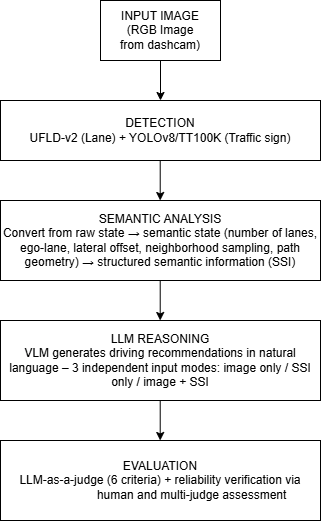
\includegraphics[
        width=0.75\textwidth,
        height=0.65\textheight,
        keepaspectratio
    ]{src-v2/figures/hinh_3_1_kien_truc.png}
    \caption{Overall architecture of the pipeline.}
    \label{fig:pipeline}
\end{figure}

In the SSI extraction module, the detection step consists of a lane-detection model and a traffic-sign-detection model, which process the same image $I$ in parallel; the semantic representation step implements the function $\Phi$ in \eqref{eq:3.1} using geometric rules and contains no learnable parameters. The recommendation generation module supplies the image and/or SSI to the VLM according to the three modes in \eqref{eq:3.3}. The evaluation stage uses LLM-as-a-Judge to score the recommendations against the rubric and compares the results with human evaluation.

\section{Model and Data Selection}

\subsection{Output Requirements and Selection Criteria}

Model selection is based on the output requirements of each module and on the deployment constraints defined in Section 3.1. The criteria are specified for each module in Sections 3.3.2--3.3.4, but they share three requirements: (i) fulfilling the function of the module in the pipeline, (ii) suiting the available resources and deployment method, and (iii) providing outputs suitable for the subsequent processing steps.

\subsection{Lane Detection}

\subsubsection*{Basis for model and data selection}

Based on the criteria above, the thesis prefers models with available pretrained checkpoints and training data suited to the problem, in order to reduce training cost and ensure reproducibility. CULane \cite{pan2018culane} is chosen as the common benchmark for comparing the models, because published results exist for UFLD-v2 \cite{qin2022ufldv2}, LaneATT \cite{tabelini2021laneatt}, and CLRNet \cite{zheng2022clrnet} (Table~\ref{tab:3.1}).

\begin{table}[H]
    \centering
    \small
    \renewcommand{\arraystretch}{1.25}
    \caption{Comparison of several lane-detection methods on CULane.}
    \label{tab:3.1}
    \begin{tabularx}{\linewidth}{
        >{\RaggedRight\arraybackslash}X
        >{\RaggedRight\arraybackslash}X
        >{\Centering\arraybackslash}p{2.2cm}
        >{\Centering\arraybackslash}p{2.2cm}
    }
        \toprule
        \textbf{Model} & \textbf{Backbone} & \textbf{F1 (\%)} & \textbf{FPS} \\
        \midrule
        LaneATT & ResNet-34 & 76.7 & 171 \\
        UFLD-v2 & ResNet-34 & 76.0 & 156 \\
        CLRNet & ResNet-34 & 79.7 & 103 \\
        CLRNet & DLA-34 & 80.5 & 94 \\
        \bottomrule
    \end{tabularx}
    \par\smallskip
    \begin{minipage}{\linewidth}
        \footnotesize\textit{Note:} The F1 and FPS values are taken from the original papers and were measured on different GPUs: LaneATT on an RTX 2080 Ti \cite{tabelini2021laneatt}, UFLD-v2 on an RTX 3090 \cite{qin2022ufldv2}, and CLRNet on a GTX 1080 Ti without TensorRT \cite{zheng2022clrnet}. Therefore, FPS is used only for reference and is not compared directly across works.
    \end{minipage}
\end{table}

In terms of benchmark results, UFLD-v2 does not achieve the highest F1, but it has two characteristics that suit the SSI extraction module. First, the model uses a row-based lane representation, which can be decoded directly into point coordinates on the lane boundaries without converting from a segmentation mask. Second, UFLD-v2 does not require NMS at inference, whereas LaneATT and CLRNet implement NMS as a CUDA extension in their official releases, which requires the CUDA Toolkit to compile \cite{laneatt2021repo,clrnet2022repo} and must be adapted to run on a CPU.

The official UFLD-v2 repository \cite{qin2022ufldv2repo} provides ResNet-34 checkpoints on three datasets: CULane, TuSimple \cite{tusimple2017}, and CurveLanes \cite{xu2020curvelanes}; the LLAMAS dataset \cite{behrendt2019llamas} has results published in \cite{qin2022ufldv2} but no corresponding checkpoint. Table~\ref{tab:3.2} compares these datasets.

\begin{table}[H]
    \centering
    \small
    \renewcommand{\arraystretch}{1.25}
    \caption{Comparison of the datasets corresponding to UFLD-v2 checkpoints.}
    \label{tab:3.2}
    \begin{tabularx}{\linewidth}{
        >{\RaggedRight\arraybackslash}p{2.4cm}
        >{\Centering\arraybackslash}p{2.0cm}
        >{\RaggedRight\arraybackslash}X
        >{\Centering\arraybackslash}p{2.6cm}
        >{\Centering\arraybackslash}p{2.4cm}
    }
        \toprule
        \textbf{Dataset} & \textbf{Images} & \textbf{Conditions} & \textbf{UFLD-v2 checkpoint} & \textbf{UFLD-v2 F1 (\%)} \\
        \midrule
        CULane & 133,235 & 9 scenario groups & Yes & 76.0 \\
        CurveLanes & 150,000 & Curved roads & Yes & 81.34 \\
        TuSimple & 6,408 & Highway, daytime & Yes & 96.22 \\
        LLAMAS & 100,042 & Highway & No & 94.95 \\
        \bottomrule
    \end{tabularx}
    \par\smallskip
    \begin{minipage}{\linewidth}
        \footnotesize\textit{Note:} The F1 values are compiled from \cite{qin2022ufldv2} and are not compared directly across datasets because of differences in data and evaluation protocol. For TuSimple, the value of 96.22\% corresponds to protocol 2; for CULane, the value of 76.0\% uses FLTTA. The nine scenario groups of CULane are: normal, crowd, dazzle light, shadow, no line, arrow, curve, crossroad, and night \cite{pan2018culane}.
    \end{minipage}
\end{table}

TuSimple and LLAMAS mainly consist of highways, CurveLanes focuses on curved roads, and LLAMAS has no official checkpoint. CULane covers nine scenario groups, including night, crossroads, curves, congestion, and difficult viewing conditions, and therefore best suits the evaluation scope of the thesis. Accordingly, the thesis uses the UFLD-v2 ResNet-34 checkpoint pretrained on CULane (published F1 of 76.0\%) and uses CULane as the image source for evaluating the SSI extraction module and for the VLM experiments.

\subsubsection*{Evaluation data and lane ground truth}

From the CULane dataset, the thesis randomly selects 200 images with a resolution of 1640 $\times$ 590 pixels to evaluate the SSI extraction module and to use in the VLM experiments in Chapter 4. Ground truth was built manually for all images according to the information fields in Table~\ref{tab:3.3}.

\begin{table}[H]
    \centering
    \small
    \renewcommand{\arraystretch}{1.25}
    \caption{Manually annotated information fields.}
    \label{tab:3.3}
    \begin{tabularx}{\linewidth}{
        >{\RaggedRight\arraybackslash}p{3.0cm}
        >{\RaggedRight\arraybackslash}X
    }
        \toprule
        \textbf{Field} & \textbf{Meaning} \\
        \midrule
        Lane count & The number of observable same-direction lanes \\
        Ego lane & Whether the ego lane output by the pipeline matches the lane the vehicle is actually in \\
        Road shape & The shape of the road \\
        Traffic signs & The number and types of observed traffic signs \\
        Hard & The difficulty level of the image and the reason \\
        \bottomrule
    \end{tabularx}
\end{table}

The ground truth was determined from the structure observable in the image rather than by directly using CULane's default labels; images with complex viewpoints or structures were reviewed manually according to the evaluation definitions of the thesis. Lane count and road shape are labeled independently of the model output, whereas the ego lane and the traffic-sign detections are labeled by visually checking the pipeline output against the image; these labels therefore evaluate the pipeline output and cannot be reused directly to evaluate another method.

\subsection{Traffic Sign Detection}

\subsubsection*{Data selection}

Unlike lane detection, there is no pretrained checkpoint available for the target traffic-sign classes, so the model must be fine-tuned on a specialized dataset whose labels include the position and class of each sign. The thesis considers five datasets: TT100K \cite{zhu2016tt100k}, GTSRB \cite{stallkamp2012gtsrb}, LISA \cite{mogelmose2012lisa}, BDD100K \cite{yu2020bdd100k}, and Mapillary \cite{ertler2020mapillary} (Table~\ref{tab:3.4}).

\begin{table}[H]
    \centering
    \small
    \renewcommand{\arraystretch}{1.25}
    \caption{Comparison of the traffic-sign datasets considered.}
    \label{tab:3.4}
    \begin{tabularx}{\linewidth}{
        >{\RaggedRight\arraybackslash}p{2.2cm}
        >{\Centering\arraybackslash}p{2.8cm}
        >{\Centering\arraybackslash}p{2.0cm}
        >{\RaggedRight\arraybackslash}X
        >{\Centering\arraybackslash}p{2.3cm}
    }
        \toprule
        \textbf{Dataset} & \textbf{Scale} & \textbf{Classes} & \textbf{Label format} & \textbf{Suitable for detection} \\
        \midrule
        TT100K & 100,000 images & 221 & Bounding box + class & Yes \\
        GTSRB & 51,839 images & 43 & Cropped image + class & No \\
        LISA & 6,610 images & 47 & Bounding box + class & Yes \\
        BDD100K & 100,000 images & 1 generic class & Bounding box + class & No \\
        Mapillary & 105,000 images & 400 & Bounding box + class & Yes \\
        \bottomrule
    \end{tabularx}
    \par\smallskip
    \begin{minipage}{\linewidth}
        \footnotesize\textit{Note:} Only 52,000 of the 105,000 Mapillary images are fully annotated.
    \end{minipage}
\end{table}

GTSRB consists only of cropped sign images and therefore has no position information, while BDD100K merges all signs into a single ``traffic sign'' class; neither meets the requirement of detection with classification. LISA has a suitable label format but is small; Mapillary's class system spans a global scope, whereas the thesis needs a fixed set of target classes. TT100K has a large scale, bounding-box labels with classes, and enough classes to select a set suited to the research scope, and it is therefore chosen as the fine-tuning data.

\subsubsection*{Model selection}

The thesis considers the YOLOv8 \cite{jocher2023yolov8} and RT-DETR \cite{zhao2024rtdetr} variants, which are detectors that support fine-tuning on bounding-box data and directly provide the position and class of objects (Table~\ref{tab:3.5}).

\begin{table}[H]
    \centering
    \small
    \renewcommand{\arraystretch}{1.25}
    \caption{Comparison of several object-detection models.}
    \label{tab:3.5}
    \begin{tabularx}{\linewidth}{
        >{\RaggedRight\arraybackslash}X
        >{\Centering\arraybackslash}p{2.2cm}
        >{\Centering\arraybackslash}p{1.7cm}
        >{\Centering\arraybackslash}p{2.2cm}
        >{\Centering\arraybackslash}p{1.9cm}
        >{\Centering\arraybackslash}p{2.0cm}
    }
        \toprule
        \textbf{Model} & \textbf{Parameters} & \textbf{GFLOPs} & \makecell{\textbf{COCO}\\\textbf{mAP50-95}\\\textbf{(\%)}} & \makecell{\textbf{CPU}\\\textbf{latency*}} & \makecell{\textbf{FPS}\\\textbf{on T4}\\\textbf{GPU**}} \\
        \midrule
        YOLOv8n & 3.2 M & 8.7 & 37.3 & 80.4 ms & --- \\
        YOLOv8s & 11.2 M & 28.6 & 44.9 & 128.4 ms & 136 \\
        YOLOv8m & 25.9 M & 78.9 & 50.2 & 234.7 ms & 97 \\
        RT-DETR-R18 & 20 M & 60.7 & 46.5 & --- & 217 \\
        RT-DETR-R34 & 31 M & 92.7 & 48.9 & --- & 161 \\
        \bottomrule
    \end{tabularx}
    \par\smallskip
    \begin{minipage}{\linewidth}
        \footnotesize\textit{Note:} The parameters, GFLOPs, mAP, and CPU latency of YOLOv8 follow the Ultralytics documentation \cite{jocher2023yolov8}; the RT-DETR figures and all T4 FPS values follow \cite{zhao2024rtdetr}. (*) CPU ONNX inference latency reported by Ultralytics; no CPU latency is published for RT-DETR. (**) FPS at batch size 1 on an NVIDIA T4 GPU with TensorRT FP16, as measured in \cite{zhao2024rtdetr}; YOLOv8n is not included in that measurement.
    \end{minipage}
\end{table}

The larger YOLOv8 variants achieve higher mAP on COCO, but their computational cost and CPU latency grow quickly; the two RT-DETR variants also have considerably more parameters and GFLOPs than YOLOv8n. Although the RT-DETR variants reach high FPS on a GPU with TensorRT, these figures do not reflect the CPU-only deployment setting of the thesis. Because the thesis prioritizes a lightweight pipeline running on a CPU (Section 3.1), YOLOv8n is chosen rather than maximizing accuracy on COCO; the latency of the variants measured on the experimental configuration is presented in Section 4.2.4.

\subsubsection*{Class scope and fine-tuning data}

TT100K contains 221 classes with an uneven sample distribution. Signs are encoded by group: prohibitory signs (``p''), mandatory signs (``i''), warning signs (``w''), and speed-limit signs (``pl''/``il'' followed by the speed value). The thesis selects 50 classes suited to the detection scope of the system instead of using all classes. Because the COCO class system does not contain these traffic-sign classes, YOLOv8n is initialized from a checkpoint pretrained on COCO and then fine-tuned on the 50-class dataset; the training configuration and results are presented in Sections 4.1.4 and 4.2.2.

The list of the 50 classes, the class codes, the semantic names, and the corresponding sign groups are presented in Table~\ref{tab:3.6}. This mapping table is used consistently in training, evaluation, and construction of the traffic-sign fields in SSI, namely the class code (\texttt{sign\_code}), the semantic name (\texttt{sign\_name}), and the sign group (\texttt{sign\_type}).

\begin{longtable}{
    >{\RaggedRight\arraybackslash}p{3.2cm}
    >{\RaggedRight\arraybackslash}p{5.0cm}
    >{\RaggedRight\arraybackslash}p{6.3cm}
}
    \caption{List of TT100K traffic-sign classes/class groups used to fine-tune YOLOv8n.}
    \label{tab:3.6} \\
    \toprule
    \textbf{Group} & \textbf{Class code} & \textbf{Semantic name} \\
    \midrule
    \endfirsthead
    \caption[]{List of TT100K traffic-sign classes/class groups used to fine-tune YOLOv8n. (continued)} \\
    \toprule
    \textbf{Group} & \textbf{Class code} & \textbf{Semantic name} \\
    \midrule
    \endhead
    \midrule
    \multicolumn{3}{r}{\footnotesize\itshape Continued on next page\ldots} \\
    \endfoot
    \bottomrule
    \endlastfoot
    Prohibitory signs & \texttt{p1} & No straight ahead \\
     & \texttt{p3} & No entry for buses \\
     & \texttt{p5} & No U-turn \\
     & \texttt{p6} & No bicycles \\
     & \texttt{p10} & No entry for motor vehicles \\
     & \texttt{p11} & No horn blowing \\
     & \texttt{p12} & No entry for motorcycles \\
     & \texttt{p13} & No entry for tractors and agricultural vehicles \\
     & \texttt{p19} & No right turn \\
     & \texttt{p23} & No left turn \\
     & \texttt{p26} & No entry for trucks \\
     & \texttt{p27} & No entry for dangerous goods vehicles \\
     & \texttt{pb} & No entry / Wrong way \\
     & \texttt{pbp} & No entry for motorized tricycles \\
     & \texttt{pn} & No parking \\
     & \texttt{pne} & No entry \\
     & \texttt{pl5}, \texttt{pl10}, \texttt{pl15}, \texttt{pl20}, \texttt{pl25}, \texttt{pl30}, \texttt{pl35}, \texttt{pl40}, \texttt{pl50}, \texttt{pl60}, \texttt{pl65}, \texttt{pl70}, \texttt{pl80}, \texttt{pl90}, \texttt{pl100}, \texttt{pl110}, \texttt{pl120} & Maximum speed limit \textit{N} km/h \\
     & \texttt{pm} & Maximum weight limit 10t \\
     & \texttt{pa} & Maximum axle weight limit 10t \\
     & \texttt{ph} & Height limit 3.5m \\
     & \texttt{pr} & End of maximum speed limit 40 km/h \\
    Mandatory signs & \texttt{pg} & Give Way \\
     & \texttt{i2} & Route for bicycles only \\
     & \texttt{i4} & Route for motor vehicles only \\
     & \texttt{i5} & Mandatory direction sign \\
    Informative signs & \texttt{ip} & Route for pedestrians and bicycles \\
     & \texttt{il50}, \texttt{il60}, \texttt{il70}, \texttt{il80}, \texttt{il90}, \texttt{il100}, \texttt{il110} & Speed advisories / Speed indicator \textit{N} km/h \\
    Warning signs & \texttt{w} & Warning sign (generic, unspecified hazard type) \\
\end{longtable}

Limiting the scope to 50 classes clearly defines the class space of the traffic-sign-detection model and keeps it consistent with the set of classes used in SSI.

\subsubsection*{Traffic-sign ground truth}

Neither CULane nor the self-collected dataset (Section 3.3.5) has traffic-sign labels under the class system of the thesis. Therefore, the traffic-sign ground truth on the two evaluation sets was built manually: for each image, the number and types of the actual signs were determined through visual review, and each detection of the module was then checked visually against the image. For each incorrect detection, the error type was also recorded: a detection on an object that is not a sign, or a detection on a real sign but with the wrong type, including the case of a sign outside the 50 classes in Table~\ref{tab:3.6}. The rules for determining correct detections, incorrect detections, and misses are presented in Section 4.1.3.

\subsection{VLM Selection}

The VLM needs to process images and text simultaneously and is used in its pretrained state through an API. NVIDIA NIM is chosen as the source of candidates because it provides API endpoints for many VLMs, with free-access options within the usage scope of this work; restricting the candidates to one platform also unifies the API-call protocol across models. Three candidates with different parameter scales are selected for screening:

\begin{itemize}
    \item \texttt{nemotron-nano-vl-8b} (8 billion parameters);
    \item \texttt{nemotron-nano-12b-v2-vl} (12 billion parameters);
    \item \texttt{ising-calibration-31b} (31 billion parameters).
\end{itemize}

The candidates are evaluated under the same API-call conditions, on the same data in the Combined mode, along three aspects: execution stability, output-format compliance, and content quality. The model chosen after screening is fixed for the whole controlled comparative experiment (Section 3.6.1); the screening results are presented in Section 4.3.1.

\subsection{Self-Collected Data and Ground Truth}

In addition to CULane, the study uses 200 frames extracted from real dashcam videos, with a resolution of 1280$\times$720 and a sampling interval of 60 to 6000 frames. This dataset is used to evaluate the generalization ability of the pipeline on data whose viewing conditions differ from CULane. The ground truth was annotated manually according to the fields in Table~\ref{tab:3.3}; the traffic-sign ground truth was built following the procedure in Section 3.3.3.

\section{Semantic Representation}

The semantic representation step converts the geometric output of the detection step into attributes that the VLM can use directly when generating recommendations. This step is designed according to four principles.

First, the attributes are selected according to the needs of the recommendation and the limitations of the VLM. The attributes retained (lane count, ego lane, vehicle offset, neighboring lanes, road shape, and traffic signs) are the information on which lane-keeping, lane-changing, or speed-adjustment recommendations depend directly, and they are also quantitative spatial relationships that general-purpose VLMs find difficult to exploit reliably from the image \cite{tong2024eyeswideshut,kamath2023whatsup}.

Second, the attributes are derived with explicit geometric rules rather than a learned model. There is no labeled dataset available for attributes such as the ego lane or the vehicle offset, and the thesis does not train an additional model for this step; geometric rules allow the attributes to be derived directly from the output of the detection step, run on a CPU, and make each value explainable.

Third, continuous quantities are discretized into meaningful labels (direction and magnitude of the offset, severity and direction of the curve), accompanied by numerical values when needed, so that the VLM receives the information in a form close to language rather than as pixel coordinates.

Fourth, each field is designed so that it can be verified against ground truth or traced back to fields that have been verified; the degree of verification of each field is evaluated in Section 4.2.3.
\subsection{Lane Semantic Extraction}

This step was designed and implemented in this work and consists of explicit rules and geometric computations, with no learnable parameters. This step converts the lane boundaries detected by UFLD-v2 into semantic attributes for the SSI representation, including the ego lane, the vehicle offset, the road shape, and the neighboring lanes.

\subsubsection*{Preprocessing: sorting the boundaries by their actual position}

$W$ and $H$ denote the image width and height, respectively, in pixels.

The input to this step is the set of boundaries

\begin{equation}
B=\{b_1,\ldots,b_n\}
\label{eq:3.4}
\end{equation}

returned by UFLD-v2. The order of the boundaries in the model output is not used to infer their actual left--right position. Because the subsequent steps need to identify pairs of spatially adjacent boundaries, the boundaries are re-sorted from left to right based on their $x$ coordinate at a reference image row $y_r$.

The reference row is determined by

\begin{equation}
y_r=\rho H,
\label{eq:3.5}
\end{equation}

where $\rho\in(0,1]$ determines the position of the reference row relative to the image height; the closer $\rho$ is to 1, the closer the reference row is to the bottom of the image. The reference row is placed near the bottom of the image but not flush against the lower edge, to avoid the region occluded by the hood or the vehicle structure.

For each boundary, the coordinate $x(y_r)$ is estimated from the points with

\begin{equation}
|y-y_r|\leq30
\label{eq:3.6}
\end{equation}

pixels. Using a neighborhood window instead of a single image row reduces the effect of sparsity or noise in the output points. If no point falls within the window, $x(y_r)$ is extrapolated with a linear model fitted to all available points of the boundary.

The boundaries are then sorted by increasing $x(y_r)$, forming a list from left to right. This list is used as the input to the step of determining the ego lane and the neighboring lanes.

\subsubsection*{Determining the ego lane}

The camera is assumed to be mounted near the horizontal center of the vehicle. The vehicle center in the image is determined by

\begin{equation}
x_v=\frac{W}{2}+o_c,
\label{eq:3.7}
\end{equation}

where $o_c$ is a horizontal calibration offset, set to 0 when no calibration information is available.

With the boundaries sorted from left to right, each pair of adjacent boundaries $(b_i,b_{i+1})$ forms a candidate gap. The gap with the smallest penalty score is chosen as the ego lane:

\begin{equation}
s_i=
\left|
\frac{x_i+x_{i+1}}{2}-x_v
\right|
\beta_i
\left(
1+0.2\frac{|w_i-w_0|}{w_0}
\right),
\label{eq:3.8}
\end{equation}

where $w_i=x_{i+1}-x_i$, $w_0=0.15W$, and $\beta_i=0.5$ if $x_v$ lies within the gap, otherwise $\beta_i=1$. The formula favors gaps whose center is close to the vehicle center, while also favoring the gap that contains the vehicle center and penalizing gaps with an unusual width.

The confidence of the ego lane is determined by the distance between the center of the selected gap and $x_v$, with heuristic levels of 0.95, 0.8, 0.6, and 0.4 corresponding to the thresholds $0.1W$, $0.25W$, $0.4W$, and all remaining cases. When only one boundary is detected, the system treats that boundary as the right boundary of the ego lane and sets the confidence to 0.5. When no boundary is detected, the system returns an empty result.

\subsubsection*{Vehicle offset}

With the ego-lane center

\begin{equation}
x_{\ell}=\frac{x_i+x_{i+1}}{2},
\label{eq:3.9}
\end{equation}

the vehicle offset is computed in pixels and as a proportion of the lane width:

\begin{equation}
\Delta x=x_v-x_{\ell}, \qquad
\Delta x_{\%}=\frac{\Delta x}{w_{\ell}}\times100,
\label{eq:3.10}
\end{equation}

where $w_{\ell}=x_{i+1}-x_i$ is the width of the ego lane. A value of $\Delta x>0$ indicates that the vehicle is offset to the right, and $\Delta x<0$ indicates an offset to the left. The system considers the vehicle to be near the lane center when $|\Delta x|<10$ pixels. The offset magnitude is labeled \textit{none} if $|\Delta x_{\%}|<10\%$, \textit{slight} if $10\%\le|\Delta x_{\%}|<30\%$, and \textit{significant} otherwise.

\begin{figure}[H]
    \centering
    \includegraphics[
        width=0.75\textwidth,
        height=0.65\textheight,
        keepaspectratio
    ]{src-v2/figures/hinh_3_2.png}
    \caption{Geometry for determining the ego lane and the vehicle offset.}
    \label{fig:offset}
\end{figure}

In Figure~\ref{fig:offset}, the two solid lines are the pair of boundaries chosen as the ego lane; the orange point is the lane center $x_{\ell}$, and the black point is the vehicle center $x_v$.

\subsubsection*{Curvature estimation}

For each boundary with at least 4 points, the $y$ coordinates are normalized by the image height, and the boundary is approximated with degree-1 and degree-2 polynomials. Let $\mathrm{MSE}_1$ and $\mathrm{MSE}_2$ be the mean squared errors of the two models. Two quantities describing curvature are computed by

\begin{equation}
\delta=\frac{\sqrt{\mathrm{MSE}_1}}{W},
\label{eq:3.11}
\end{equation}

\begin{equation}
\eta=
\begin{cases}
0, & \mathrm{MSE}_1\leq4,\\[4pt]
\max\left(0,\dfrac{\mathrm{MSE}_1-\mathrm{MSE}_2}{\mathrm{MSE}_1}\right),
& \mathrm{MSE}_1>4.
\end{cases}
\label{eq:3.12}
\end{equation}

Here, $\delta$ measures the deviation from a straight line, and $\eta$ measures the improvement obtained with the degree-2 model. $\eta$ is used only for boundaries with at least 10 points and $\mathrm{MSE}_1>4$.

The curve direction is determined from the horizontal shift of the boundaries. For each boundary $b_j$, let $\bar{x}_j^{\mathrm{bot}}$ and $\bar{x}_j^{\mathrm{top}}$ be the mean horizontal coordinates of the 20\% of points closest to the bottom and the 20\% of points closest to the top of that boundary. The normalized horizontal shift is computed by

\begin{equation}
\sigma=\frac{1}{W\,|B'|}\sum_{b_j\in B'}\left(\bar{x}_j^{\mathrm{bot}}-\bar{x}_j^{\mathrm{top}}\right),
\label{eq:3.13}
\end{equation}

where $B'$ is the set of boundaries with at least 4 points that span at least 5\% of the image height.

The quantities $\overline{\delta}$, $\overline{\eta}$, the proportion of straight boundaries $r_{\mathrm{straight}}$, and the horizontal shift $\sigma$ are aggregated to classify the road shape and the curve direction.

\subsubsection*{Classification of road shape and curve direction}

The road shape is classified into three levels: straight, gentle curve, and sharp curve:

\begin{equation}
c=
\begin{cases}
\text{straight},
&
\overline{\delta}<0.02
\land
\overline{\eta}<0.3
\land
r_{\mathrm{straight}}>0.5,
\\[4pt]
\text{sharp curve},
&
\overline{\delta}\geq0.06,
\\[4pt]
\text{gentle curve},
&
\text{otherwise},
\end{cases}
\label{eq:3.14}
\end{equation}

where $r_{\mathrm{straight}}\in[0,1]$ is the proportion of boundaries determined to be straight; a boundary is considered straight when $\mathrm{MSE}_1<1000$ pixels$^2$, i.e., its root-mean-square deviation from the fitted straight line is below about 32 pixels. For curved roads, the curve direction is determined by the sign of the horizontal shift $\sigma$ in \eqref{eq:3.13}: $\sigma>0$ corresponds to a right curve and $\sigma<0$ to a left curve. Combining the severity and direction of the curve, the system produces the labels gentle left curve, gentle right curve, sharp left curve, and sharp right curve.

\subsubsection*{Lane count}

The number of lanes is determined as the number of detected lane boundaries minus one, since $n$ adjacent boundaries form $n-1$ lane intervals.

\subsubsection*{Note on the parameters}

The thresholds and coefficients in Section 3.4.1 are heuristic parameters, including: the penalty coefficient 0.2 and the reference lane width $w_0=0.15W$ in \eqref{eq:3.8}; the confidence levels 0.95/0.8/0.6/0.4; the 10-pixel threshold for the near-center state; the 10\% and 30\% thresholds for the offset magnitude; the 20\% share of points near the bottom/top and the minimum boundary length of 5\% of the image height in \eqref{eq:3.13}; the threshold $\mathrm{MSE}_1<1000$ for a straight boundary; and the thresholds on $\overline{\delta}$, $\overline{\eta}$, and $r_{\mathrm{straight}}$ in \eqref{eq:3.14}. They were chosen manually through visual inspection of sample images, with the aim of discretizing continuous geometric quantities into a small number of levels that are easy for the VLM to interpret. These parameters were not optimized by searching over the ground truth. The sensitivity of the results to each parameter has not been examined and is a limitation of the module.

\subsection{Traffic Sign Semantic Extraction}

Traffic-sign semantics are extracted from the output of YOLOv8n. For each input image, the model returns the detections with a confidence of 0.5 or higher, where each detection consists of a bounding box, a confidence, and a class code. The class code is kept in the \texttt{sign\_code} field and mapped to a semantic name (\texttt{sign\_name}) and a sign group (\texttt{sign\_type}) according to Table~\ref{tab:3.6}. The extraction consists of three steps: filtering the detections, mapping the class codes, and determining the relative position of each sign.

The relative position is determined from the horizontal coordinate of the bounding-box center:

\begin{equation}
relative\_position=
\begin{cases}
\text{left}, & x_c<0.33W,\\
\text{right}, & x_c>0.66W,\\
\text{center}, & \text{otherwise},
\end{cases}
\label{eq:3.15}
\end{equation}

where $x_c$ is the center coordinate of the bounding box and $W$ is the image width. This is a 2D heuristic intended to add positional information to SSI; it is not a quantity that is learned or calibrated from ground truth.

\subsection{SSI Construction}

The lane and traffic-sign semantic extraction results are normalized into a single Structured Semantic Information (SSI) structure in JSON form for each image (Figure~\ref{fig:ssiflow}). This structure is used as the input to the VLM in the SSI-only and Combined modes and also serves as the intermediate representation in the evaluation experiments.

\begin{figure}[H]
    \centering
    \includegraphics[
        width=0.75\textwidth,
        height=0.65\textheight,
        keepaspectratio
    ]{src-v2/figures/hinh_3_3.png}
    \caption{Data-transformation flow in the semantic representation step.}
    \label{fig:ssiflow}
\end{figure}

SSI consists of six groups of information: lane count, ego-lane position and confidence, vehicle offset, neighboring lanes, road shape, and traffic signs. The fields were selected to retain the information that directly serves situation analysis and driving-recommendation generation.

Intermediate results are normalized into SSI only when they correspond to an information field defined in Table~\ref{tab:3.7}. This organization keeps the semantic representation minimal while still providing the information needed for the VLM's reasoning step.

An example of an actual SSI:

\begin{adjustwidth}{0.04\linewidth}{0.04\linewidth}
\begin{framed}
\footnotesize
\begin{verbatim}
{
  "lane_count": 3,
  "order": "left to right",
  "ego_lane": {
    "position": "2/3",
    "confidence": 0.8
  },
  "vehicle_offset": {
    "direction": "right",
    "magnitude": "significant",
    "offset_percent": 31.2
  },
  "neighbor_lanes": {
    "left_count": 1,
    "right_count": 1
  },
  "road_shape": {
    "type": "straight",
    "severity": "none",
    "direction": null
  },
  "traffic_signs": {
    "detected": [
      { "sign_code": "i5", "confidence": 0.80,
        "bbox": [495, 324, 516, 342], "relative_position": "left",
        "sign_name": "Mandatory direction sign",
        "sign_type": "Mandatory Sign"},
      { "sign_code": "i4", "confidence": 0.74,
        "bbox": [952, 311, 978, 336], "relative_position": "center",
        "sign_name": "Route for motor vehicles only",
        "sign_type": "Mandatory Sign" }
    ]
  }
}
\end{verbatim}
\end{framed}
\end{adjustwidth}

In the example above, the vehicle is in lane 2 of 3, offset 31.2\% to the right of the lane center, has one neighboring lane on each side, the road is straight, and two signs are detected on the left and in the center of the image.

\begin{table}[!htbp]
    \centering
    \setstretch{1.5}
    \small
    \renewcommand{\arraystretch}{1.25}
    \caption{Summary of the information fields in SSI.}
    \label{tab:3.7}
    \begin{tabularx}{\linewidth}{
        >{\RaggedRight\arraybackslash}p{3.6cm}
        >{\RaggedRight\arraybackslash}p{2.8cm}
        >{\RaggedRight\arraybackslash}p{3.0cm}
        >{\RaggedRight\arraybackslash}X
    }
        \toprule
        \textbf{Field} & \textbf{Source} & \textbf{Representation} & \textbf{Purpose} \\
        \midrule
        \texttt{lane\_count} & Semantic representation & Integer & Number of observed lanes \\
        \texttt{order} & Semantic representation & Fixed string (\texttt{left to right}) & Direction of lane numbering, e.g., from left to right \\
        \texttt{ego\_lane} (\texttt{position}, \texttt{confidence}) & Semantic representation & Position as \texttt{k/n} and heuristic confidence & Identifies the lane the vehicle is in \\
        \texttt{vehicle\_offset} (\texttt{direction}, \texttt{magnitude}, \texttt{offset\_percent}) & Derived from \texttt{ego\_lane} and the boundary coordinates & Offset direction and percentage of the lane width & Describes the vehicle's position within the lane \\
        \texttt{neighbor\_lanes} (\texttt{left\_count}, \texttt{right\_count}) & Derived from \texttt{lane\_count} and \texttt{ego\_lane} & Integer on each side & Describes the observed neighboring lanes \\
        \texttt{road\_shape} (\texttt{type}, \texttt{severity}, \texttt{direction}) & Semantic representation & Classification label & Describes the road shape and curve direction \\
        \texttt{traffic\_signs} (\texttt{sign\_code}, \texttt{sign\_name}, \texttt{sign\_type}, \texttt{confidence}, \texttt{bbox}, \texttt{relative\_position}) & YOLOv8n & List of detections & Adds information about traffic signs and traffic rules \\
        \bottomrule
    \end{tabularx}
\end{table}

This SSI structure is also used as the field template in the experiment in Section 4.5.1, in which the VLM is asked to extract the corresponding fields directly from the image by itself for comparison with the pipeline's results. SSI is not provided to the VLM in that experiment.

\section{Recommendation Generation Module}

The recommendation generation module uses the VLM in its pretrained state through an API, without changing the model parameters; therefore, recommendation quality depends on how the information and the requirements are put into the prompt. The prompt design has three goals: (i) limiting unsubstantiated content by constraining the model to use only the evidence present in the input, i.e., an inference-time grounding mechanism to reduce hallucination \cite{ji2023hallucination,lewis2020rag}; (ii) ensuring a fair comparison between modes by keeping every component of the prompt fixed except the information source and the instructions for using that source; and (iii) producing a uniformly structured output that can be scored with the same rubric.

SSI is inserted into the prompt as raw JSON rather than being converted into sentences. This keeps the field names and the hierarchical structure of SSI intact, avoids adding the author's interpretation to the VLM's input, and makes it possible to trace exactly what information the model received.

The prompt is designed so that the VLM performs the same task in the three input modes: Image-only, SSI-only, and Combined. The request structure and the generation flow are illustrated in Figure~\ref{fig:promptstruct}.

\begin{figure}[H]
    \centering
    \includegraphics[
        width=0.75\textwidth,
        height=0.65\textheight,
        keepaspectratio
    ]{src-v2/figures/hinh_3_4.png}
    \caption{Request structure and recommendation-generation flow of the VLM.}
    \label{fig:promptstruct}
\end{figure}

\subsection{Prompt Design Principles}

All three modes share a common instruction block that defines the role of the VLM, the task, the principles for using evidence, and the output requirements, in order to remove differences in task requirements between the modes. The VLM may use only the evidence present in the input: for the image, observable content; for SSI, the information represented in the JSON. The fact that an object does not appear in the detection results is not treated as evidence that the object does not exist, because the detection modules may miss objects.

In the Combined mode, SSI is produced from detection results and may therefore not be fully consistent with the image. The prompt requires the model to use the image when there is clear visual evidence, and to use SSI for information that is difficult to determine reliably from the image, such as the lane configuration, the ego lane, the offset, and the traffic signs. When the two sources clearly conflict, the model uses the source with stronger direct evidence for each piece of information, briefly states the uncertainty if it affects the decision, and does not assume that SSI is always correct.

\subsection{Design of the Input Modes}

The prompt of each mode consists of three blocks concatenated in a fixed order:

\begin{equation}
P_m = P_{\mathrm{common}} \oplus B_m \oplus P_{\mathrm{out}}
\label{eq:3.16}
\end{equation}

where $P_{\mathrm{common}}$ is the common instruction block (role, task, evidence-use principles, and hallucination control) and $P_{\mathrm{out}}$ is the output-format block; these two blocks are identical in all three modes. $B_m$ is the mode-specific block for mode $m$, which contains the instructions for using the information source and the SSI data, if any; this block differs across modes because each mode receives a different information source:

\begin{itemize}
    \item \textbf{Image-only:} the RGB image is the only source of information; the model acknowledges uncertainty when information cannot be determined from the image.
    \item \textbf{SSI-only:} SSI in JSON form is the only source of information and is treated as perception output, not ground truth; missing fields or an empty detection list are not interpreted as the object not existing.
    \item \textbf{Combined:} the model receives both the image and SSI, together with the combination and conflict-handling rules in Section 3.5.1.
\end{itemize}

Each prompt $P_m$ is fixed throughout the experiments and does not change between images or calls. Therefore, the differences between modes reflect the effect of the whole input package, consisting of the information source and the instructions for using that source, and not the SSI data alone. The full text of the prompt is presented in Appendix~\ref{app:prompt}.

\subsection{Output Requirements and Generation Parameters}

To give the results a uniform structure across modes, the prompt specifies that the output consists of three parts: \textbf{Situation}, \textbf{Recommendation}, and \textbf{Safety note}. The output-structure requirement is placed at the end of the prompt content. This arrangement is based on studies of the effect of information position in the context of language models, which show that the position of information can affect how well the model uses it \cite{liu2024lostinmiddle}. In this thesis, the position of the output requirement is kept fixed and is not treated as an experimental variable.

For each mode, the system sends one API request to the VLM, containing the prompt content, the image data (for the modes that use the image), and the generation parameters. The parameters \texttt{temperature}, \texttt{top\_p}, \texttt{max\_tokens}, and \texttt{frequency\_penalty} keep the same values for every request throughout the experiments and are not experimental variables (Table~\ref{tab:3.8}).

\begin{table}[H]
    \centering
    \small
    \renewcommand{\arraystretch}{1.25}
    \caption{API call configuration used in the recommendation-generation experiments.}
    \label{tab:3.8}
    \begin{tabularx}{\linewidth}{
        >{\RaggedRight\arraybackslash}X
        >{\Centering\arraybackslash}p{3.5cm}
    }
        \toprule
        \textbf{Parameter} & \textbf{Value} \\
        \midrule
        \texttt{max\_tokens} & 400 \\
        \texttt{temperature} & 0.2 \\
        \texttt{top\_p} & 0.7 \\
        \texttt{frequency\_penalty} & 0.4 \\
        \texttt{timeout} & 120 s/request \\
        Image compression before Base64 encoding & $\le$ 150 KB \\
        \bottomrule
    \end{tabularx}
\end{table}

The generated recommendations are used as the input to the evaluation step in Section 3.6.

\section{Method for Evaluating the Change in Recommendation Quality When SSI Is Added}

This section presents the method for evaluating the change in the quality of the VLM's recommendations when structured semantic information (SSI) is added. It covers the design of the comparison conditions, the criteria for evaluating recommendation quality, and the method for quantifying and testing the change between conditions.

\subsection{Controlled Comparative Experiment Design}

The controlled comparative experiment is designed to test the research hypothesis: \textit{adding SSI to the input changes the quality of the VLM's driving recommendations compared with using only the image}. The components of the design are:

\begin{itemize}
    \item \textbf{Independent variable:} the input mode $c \in \{c_1, c_2, c_3\}$ according to \eqref{eq:3.3}.
    \item \textbf{Dependent variables:} the scores of the six criteria $s_{i,m,k}$ and the aggregate score $S_{i,m}$ according to \eqref{eq:3.2}.
    \item \textbf{Control variables:} the input image, the VLM, the common instruction block and output requirements of the prompt, the generation configuration, the judge, and the scoring rubric.
    \item \textbf{Unit of analysis:} the image; the three modes of the same image form one paired set of observations.
\end{itemize}

For each image, the VLM is run independently in all three modes (Section 3.5.2) with the same common instruction block, output requirements, and API call configuration, so the results across modes form paired observations per image. The recommendations of the three modes for the same image are scored by the judge in the same call (Section 3.6.3). The Image-only -- Combined pair most clearly shows the effect of adding SSI, because both modes receive the image and differ only in that the Combined mode is additionally given SSI together with the instructions for using it; the SSI-only mode indicates how much information SSI alone provides and supports the interpretation of the results.

\subsection{Evaluation Criteria and Rating Scale}

Output quality is evaluated with a six-criterion rubric reflecting two groups of aspects: understanding the traffic situation and the ability to form decision-support content (Table~\ref{tab:3.9}).

\begin{table}[H]
    \centering
    \small
    \renewcommand{\arraystretch}{1.25}
    \caption{Criteria for evaluating the quality of VLM outputs.}
    \label{tab:3.9}
    \begin{tabularx}{\linewidth}{
        >{\RaggedRight\arraybackslash}p{3.0cm}
        >{\RaggedRight\arraybackslash}p{3.8cm}
        >{\RaggedRight\arraybackslash}X
    }
        \toprule
        \textbf{Group} & \textbf{Criterion} & \textbf{What is evaluated} \\
        \midrule
        Situation understanding & Situation understanding & How correctly the road condition, traffic, and related hazards are understood. \\
         & Road geometry understanding & How correctly the road geometry, lanes, boundaries, and neighboring lanes are recognized. \\
         & Ego-lane position & How correctly the ego lane and the vehicle's offset are determined when evidence is available. \\
         & Signs and rules & How correctly signs, signals, and rules supported by evidence are recognized. \\
        Decision support & Driving recommendation & How appropriate, necessary, safe, and justified the proposed action is. \\
         & Safety considerations & How correctly the relevant risks are identified and how well they are tied to the situation. \\
        \bottomrule
    \end{tabularx}
\end{table}

The six criteria are derived from the output task required by the prompt (Section 3.5). The first four criteria correspond to the content the model is required to recognize in order to understand the situation; the last two criteria correspond to the Recommendation and Safety note parts. The criteria apply equally to every mode, regardless of whether the mode uses SSI.

Each criterion is scored on a 1--5 scale with equal weights. The descriptions of the score levels are presented in Table~\ref{tab:3.10}.

\begin{table}[H]
    \centering
    \small
    \renewcommand{\arraystretch}{1.25}
    \caption{Description of the rating scale.}
    \label{tab:3.10}
    \begin{tabularx}{\linewidth}{
        >{\Centering\arraybackslash}p{1.2cm}
        >{\RaggedRight\arraybackslash}X
    }
        \toprule
        \textbf{Score} & \textbf{Description} \\
        \midrule
        5 & Correct and clearly justified; no significant errors. \\
        4 & Mostly correct; only minor, non-critical errors or omissions. \\
        3 & Partially correct; notable errors or omissions, but the main understanding is still usable. \\
        2 & Serious errors that affect situation understanding or the driving decision. \\
        1 & Incorrect, unjustified, or unusable. \\
        \bottomrule
    \end{tabularx}
\end{table}

The judge uses the original image as the visual reference to check the correctness of the statements in the recommendation. Each mode is scored separately: the judge is instructed not to compare modes when scoring each criterion, and not to penalize a mode for lacking information that its input did not provide.

\subsection{Evaluation and Verification Protocol}

\begin{figure}[H]
    \centering
    \includegraphics[
        width=0.75\textwidth,
        height=0.65\textheight,
        keepaspectratio
    ]{src-v2/figures/hinh_3_6.png}
    \caption{LLM-as-a-Judge evaluation flow.}
    \label{fig:judgeflow}
\end{figure}

Each LLM-as-a-Judge call corresponds to one image and consists of four components, the first three of which are illustrated in Figure~\ref{fig:judgeflow}: (i) the reference image, which is the same image provided to the VLM; (ii) the recommendations to be compared on that image, namely the recommendations of the three input modes in the main experiment (Section 4.3.2), the recommendations of the candidate models in the screening step (Section 4.3.1), or the recommendations of the prompt versions (Section 4.5.2); (iii) the scoring prompt, consisting of the scoring instructions and the six-criterion rubric with the 1--5 scale in Section 3.6.2; and (iv) the judge's generation configuration, consisting of the temperature (where applicable) and the maximum number of output tokens (Section 4.1.4). For each recommendation, the judge returns the scores of the six criteria together with a short justification for each criterion in JSON form. The exception is the comparison with human evaluation in Section 4.4, in which each of the three judges independently scores only the Combined-mode recommendation of each image.

This joint scoring ensures that the three input modes of the same image are evaluated under the same conditions, namely the same reference image, the same scoring instructions, and the same judge inference pass, consistent with the paired comparison design in Section 3.6.1. Because the absolute scores of LLM-as-a-Judge may depend on the scoring context, the thesis compares scores between modes only within the same scoring session and does not compare absolute scores across different scoring sessions. Here, a scoring session is one pass in which the judge scores a fixed set of outputs for all images with the same scoring prompt and configuration.

Three models, Gemini \cite{geminiteam2024}, GPT-5 Mini, and DeepSeek, are used as judges. Gemini is used as the judge from the VLM screening step onward (Section 4.3.1); afterwards, all three judges are compared with human evaluation on the same set of recommendations and the same rubric to confirm the choice of the primary judge. Gemini is the primary judge for the analyses over the whole dataset; GPT-5 Mini and DeepSeek are additional judges on the same data and rubric, used to check the stability of the results when the judge changes.

The agreement between each judge and human evaluation is checked on 20 randomly selected images, using the recommendations of the Combined mode, corresponding to 120 score pairs (20 images $\times$ 6 criteria) per judge. The agreement and correlation metrics are defined in Table~\ref{tab:4.4}; the comparison results are presented in Section 4.4.

\subsection{Quantifying the Change and Statistical Testing}

The aggregate score $S_{i,m}$ of an output is computed according to \eqref{eq:3.2}. The change when SSI is added is defined as:

\begin{equation}
\Delta_i=S_{i,c_3}-S_{i,c_1}
\label{eq:3.17}
\end{equation}

and the mean change over $N$ images as:

\begin{equation}
\overline{\Delta}=\frac{1}{N}\sum_{i=1}^{N}\Delta_i
\label{eq:3.18}
\end{equation}

$\overline{\Delta}$ expresses the change directly on the 1--5 scale. For example, according to the primary judge, the mean score increases from 3.32 (Image-only) to 3.97 (Combined), corresponding to $\overline{\Delta}=+0.65$.

For each pair of modes $(a,b)$ and each image $i$, the paired difference is defined as $d_i^{(a,b)} = S_{i,a} - S_{i,b}$, following the convention in Section 4.1.3 (the first mode of the pair minus the second). Because the evaluation scores are ordinal data on a 1--5 scale, measured repeatedly on the same image and not guaranteed to be normally distributed, the thesis uses the two-sided Wilcoxon signed-rank test with the hypotheses:

\begin{equation}
H_0: \operatorname{median}\big(d^{(a,b)}\big) = 0, \qquad H_1: \operatorname{median}\big(d^{(a,b)}\big) \neq 0
\label{eq:3.19}
\end{equation}

Rejecting $H_0$ means that the scores of mode $b$ differ systematically from those of mode $a$ on the same set of images. The test is performed for all three pairs of modes $(c_1,c_2)$, $(c_1,c_3)$, and $(c_2,c_3)$ for each judge. The significance level of 0.05 is Bonferroni-corrected for the total number of comparisons (9 comparisons for 3 pairs $\times$ 3 judges, threshold 0.0056). In addition to the $p$-value, the effect size is reported with Cohen's $d_z = \bar{d}/s_d$ computed on $d_i^{(a,b)}$ (Section 4.1.3); a negative $d_z$ therefore means that mode $a$ scores lower than mode $b$. Because $\Delta_i = -d_i^{(c_1,c_3)}$, an improvement when SSI is added ($\overline{\Delta} > 0$) corresponds to a negative $d_z$ for the pair $(c_1,c_3)$; when only the magnitude of an effect is discussed, it is reported as $|d_z|$. Among the three pairs, the pair $(c_1,c_3)$ most clearly reflects the change when SSI is added; the pairs involving $c_2$ are used for reference and to support interpretation. Per-criterion analyses are performed to clarify the role of each information source in the VLM's input.

\chapter{Experiments and Results}

This chapter presents the setup and results of the experiments on the system, organized by the main components of the pipeline. Section 4.1 describes the models, data, evaluation metrics, and configuration used consistently across the experiments. Section 4.2 evaluates the SSI extraction module. Section 4.3 evaluates the candidate VLMs and compares recommendation quality across the three input modes. Section 4.4 compares the LLM-as-a-Judge evaluation results with human evaluation. Section 4.5 presents two supplementary experiments that verify the VLM's ability to self-extract semantic information and evaluate the influence of the prompt design.

The local execution environment of the SSI extraction module consists of:

\begin{itemize}
    \item \textbf{Hardware:}
    \begin{itemize}
        \item Device: Dell Inspiron 5515.
        \item Processor: AMD Ryzen 5 5500U with Radeon Graphics (6 cores / 12 threads).
        \item Memory: 16 GB RAM.
    \end{itemize}
    \item \textbf{Software:}
    \begin{itemize}
        \item Operating system: Windows 11 Pro (64-bit).
        \item Programming language: Python 3.9.
    \end{itemize}
\end{itemize}

The VLM calls are made through NVIDIA NIM, while the LLM-as-a-Judge models are called through the respective API of each provider.

\section{Experimental Setup}

\subsection{Models Used}

The models used in the experiments (Table~\ref{tab:4.1}) include UFLD-v2 for lane detection, YOLOv8n for traffic sign detection, three candidate VLMs for the screening and recommendation-generation stages (Section 3.3.4), and three judges, Gemini, GPT-5 Mini, and DeepSeek.

\begin{table}[H]
    \centering
    \footnotesize
    \renewcommand{\arraystretch}{1.25}
    \caption{Models and their roles in the experiments.}
    \label{tab:4.1}
    \begin{tabularx}{\linewidth}{
        >{\RaggedRight\arraybackslash}p{4.0cm}
        >{\RaggedRight\arraybackslash}p{3.2cm}
        >{\Centering\arraybackslash}p{1.8cm}
        >{\Centering\arraybackslash}X
        >{\Centering\arraybackslash}p{2.4cm}
    }
        \toprule
        \textbf{Model} & \textbf{Role} & \textbf{Status} & \textbf{Training/ initialization data} & \textbf{Experiments} \\
        \midrule
        UFLD-v2 & Lane detection & Pretrained & CULane & 4.2.1, 4.2.3, 4.2.4, 4.5.1 \\
        YOLOv8n & Traffic sign detection & Fine-tuned & TT100K & 4.2.2, 4.2.3, 4.2.4 \\
        \seqsplit{ising-calibration-31b} & Candidate VLM & API & --- & 4.3.1, 4.3.2, 4.3.3, 4.4, 4.5.1, 4.5.2 \\
        \seqsplit{nemotron-nano-vl-8b} & Candidate VLM & API & --- & 4.3.1 \\
        \seqsplit{nemotron-nano-12b-v2-vl} & Candidate VLM & API & --- & 4.3.1 \\
        Gemini & LLM-as-a-Judge & API & --- & 4.3.1, 4.3.2, 4.3.3, 4.4, 4.5.2 \\
        GPT-5 Mini & LLM-as-a-Judge & API & --- & 4.3.2, 4.3.3, 4.4 \\
        DeepSeek & LLM-as-a-Judge & API & --- & 4.3.2, 4.3.3, 4.4 \\
        \bottomrule
    \end{tabularx}
    \par\smallskip
    \begin{minipage}{\linewidth}
        \footnotesize\textit{Note:} UFLD-v2 and YOLOv8n also produce the SSI used as input in the experiments of Sections 4.3--4.5. ---: not applicable; these models are used as pretrained black-box models through APIs, and their training data are not disclosed.
    \end{minipage}
\end{table}

\subsection{Experimental Data}

The experiments use three main groups of data: TT100K for fine-tuning the traffic-sign-detection model, CULane for evaluating lane detection and for the VLM experiments, and self-collected dashcam data for evaluation on data outside CULane.

For TT100K, YOLOv8n is fine-tuned with the class scope and label-mapping rules presented in Section 3.3.3. The data are split into 85\% for the training set and 15\% for the validation set.

For CULane, 200 images were randomly selected, comprising 176 Normal images and 24 Hard images (Figure~\ref{fig:normalhard}). The Hard group consists of images whose lane markings are unclear or whose lane structure is difficult to determine, such as in parking garages, at intersections, in congestion, or at merging points; the remaining images belong to the Normal group. The Hard group was assigned ground truth according to the observed lane structure instead of defaulting to a no-lane label. The details of image selection and labeling are presented in Section 3.3.2.

\begin{figure}[H]
    \centering
    \includegraphics[
        width=0.75\textwidth,
        height=0.65\textheight,
        keepaspectratio
    ]{src-v2/figures/hinh_4_1.png}
    \caption{Examples of images labeled Normal and Hard. (a) Normal image. (b) Hard image.}
    \label{fig:normalhard}
\end{figure}

The self-collected data consist of 200 dashcam images, independent of CULane, used to evaluate the pipeline on data outside the main evaluation set. The characteristics and construction procedure of this dataset are presented in Section 3.3.5.

The data groups and the relationships between the input data, the outputs, and the main experiments are illustrated in Figure~\ref{fig:ch4flow}.

\begin{figure}[H]
    \centering
    \includegraphics[
        width=0.75\textwidth,
        height=0.65\textheight,
        keepaspectratio
    ]{src-v2/figures/hinh_4_2.png}
    \caption{Data flow across the experiments in Chapter 4.}
    \label{fig:ch4flow}
\end{figure}

\subsection{Evaluation Metrics}

The evaluation metrics are selected for each experiment (Table~\ref{tab:4.2}, Table~\ref{tab:4.3}, and Table~\ref{tab:4.4}).

\begin{table}[H]
    \centering
    \small
    \renewcommand{\arraystretch}{1.25}
    \caption{Evaluation metrics for lane semantic extraction.}
    \label{tab:4.2}
    \begin{tabularx}{\linewidth}{
        >{\RaggedRight\arraybackslash}p{3.8cm}
        >{\RaggedRight\arraybackslash}X
    }
        \toprule
        \textbf{Metric} & \textbf{Definition} \\
        \midrule
        Lane Count Accuracy & The proportion of images for which the module correctly determines the lane count, out of all evaluated images. \\
        Lane Count MAE & The mean absolute error between the predicted lane count and the actual lane count. \\
        Lane Count Precision & The proportion of correctly identified lanes out of the total actual lanes plus the lanes that were falsely added, wrongly merged, or taken from the opposite direction. \\
        Ego Lane Accuracy & The proportion of images for which the ego-lane position is correctly determined, out of all evaluated images. \\
        Road Shape Accuracy & The proportion of images for which the road shape is correctly classified among the five shape classes defined in Chapter 3. \\
        \bottomrule
    \end{tabularx}
\end{table}

\begin{table}[H]
    \centering
    \small
    \renewcommand{\arraystretch}{1.25}
    \caption{Evaluation metrics for traffic-sign detection.}
    \label{tab:4.3}
    \begin{tabularx}{\linewidth}{
        >{\RaggedRight\arraybackslash}p{3.8cm}
        >{\RaggedRight\arraybackslash}X
    }
        \toprule
        \textbf{Metric} & \textbf{Definition} \\
        \midrule
        Precision & The proportion of correct detections out of all detections made by the pipeline. \\
        Recall & The proportion of actual signs correctly detected out of all actual signs eligible for evaluation. \\
        F1-score & A composite metric reflecting the balance between Precision and Recall. \\
        Classification Accuracy & The proportion of detections with the correct sign type out of all detections that correspond to an actual sign by visual review (regardless of class). \\
        \bottomrule
    \end{tabularx}
\end{table}

A detection is considered correct when, by visual review, the bounding box identified by the model actually contains a sign and the predicted label matches the actual label of that sign.

\textbf{Recommendation-quality evaluation:} six criteria, namely Situation understanding, Road geometry understanding, Ego-lane position, Signs and rules, Driving recommendation, and Safety considerations. Each criterion is scored on a 1--5 scale following the description of each score level presented in Section 3.6.2 (Table~\ref{tab:3.10}).

\begin{table}[H]
    \centering
    \small
    \renewcommand{\arraystretch}{1.25}
    \caption{Evaluation metrics for agreement between LLM-as-a-Judge and humans.}
    \label{tab:4.4}
    \begin{tabularx}{\linewidth}{
        >{\RaggedRight\arraybackslash}p{3.8cm}
        >{\RaggedRight\arraybackslash}X
    }
        \toprule
        \textbf{Metric} & \textbf{Definition} \\
        \midrule
        Exact agreement & The proportion of judge--human score pairs with the same score on the same criterion for the same image. \\
        Agreement within $\pm$1 & The proportion of judge--human score pairs that differ by no more than 1 point on the same criterion for the same image. \\
        Pearson correlation & The degree of linear correlation between the judge's and the human's mean score over the six criteria, across the 20 evaluated images. \\
        \bottomrule
    \end{tabularx}
\end{table}

The formal definitions of the quantitative metrics used throughout Chapter 4, with $N$ the number of evaluated samples, $y_i$/$\hat{y}_i$ the actual/predicted value of sample $i$, $TP$/$FP$/$FN$ the numbers of correct detections/incorrect detections/misses, and $\mathbb{I}[\cdot]$ the indicator function, which equals 1 when the condition in brackets holds and 0 otherwise:

\[
\text{Accuracy} = \frac{1}{N}\sum_{i=1}^{N} \mathbb{I}[y_i = \hat{y}_i], \qquad \text{MAE} = \frac{1}{N}\sum_{i=1}^{N} |y_i - \hat{y}_i|
\]

\[
\text{Precision} = \frac{TP}{TP + FP}, \qquad \text{Recall} = \frac{TP}{TP + FN}, \qquad \text{F1} = \frac{2 \cdot \text{Precision} \cdot \text{Recall}}{\text{Precision} + \text{Recall}}
\]

For two paired samples $x$ (e.g., the scores of mode A) and $y$ (the scores of mode B) over the same $N$ images, $d_i=x_i-y_i$ is the difference between the two conditions on image $i$. The standardized effect size for paired data is computed with Cohen's $d_z$:

\[
\text{Cohen's } d_z = \frac{\bar{d}}{s_d},
\qquad
\bar{d} = \frac{1}{N}\sum_{i=1}^{N}d_i,
\qquad
s_d = \sqrt{\frac{1}{N-1}\sum_{i=1}^{N}(d_i-\bar{d})^2}.
\]

The sign of $d_z$ depends on the order of the two conditions in the comparison; a negative value indicates that the mean score of the first condition is lower than that of the second condition. The magnitude $|d_z|$ is interpreted with Cohen's conventional thresholds of 0.2 (small), 0.5 (medium), and 0.8 (large) \cite{cohen1988power}. Values reported as $a \pm b$ in the result tables denote the mean $\pm$ standard deviation over the evaluated images.

\[
r_{\text{Pearson}} = \frac{\sum_{i=1}^{N} (x_i - \bar{x})(y_i - \bar{y})}{\sqrt{\sum_{i=1}^{N} (x_i - \bar{x})^2} \sqrt{\sum_{i=1}^{N} (y_i - \bar{y})^2}}
\]

The two judge--human agreement metrics in Table~\ref{tab:4.20} are computed directly from $N$ score pairs $(h_i, j_i)$ (human, judge) on the same criterion and the same image: Exact agreement $= \frac{1}{N}\sum_{i=1}^{N}\mathbb{I}[h_i = j_i]$; Agreement within $\pm 1$ $= \frac{1}{N}\sum_{i=1}^{N}\mathbb{I}[|h_i - j_i| \le 1]$.

\subsection{Experimental Configuration}

The configurations that are shared or that directly affect the reproducibility of the experiments are summarized here.

For the detection step, UFLD-v2 uses the CULane configuration and checkpoint presented in Section 3.3.2; the reference-row position parameter is set to $\rho=0.919$, determined from the proportion of the image region still visible above the edge of the hood in the CULane images. This is a geometric characteristic of the camera mounting and does not use any ground-truth information. YOLOv8n uses the checkpoint fine-tuned on TT100K and the standard confidence threshold of 0.5 during traffic-sign evaluation.

YOLOv8n was fine-tuned on a Kaggle GPU with 640 $\times$ 640 input images, a batch size of 83, the SGD optimizer (initial learning rate 0.01, final learning-rate factor 0.01, momentum 0.937, weight decay 0.0005, 3 warm-up epochs), a maximum of 100 epochs with early stopping (patience = 30), and the default Ultralytics data-augmentation parameters.

The VLMs are called through NVIDIA NIM with the configuration in Table~\ref{tab:3.8} (Section 3.5.3), shared by the three candidate models and the three input modes; the main experiment keeps the sample count and the per-image pairing order fixed across the three modes. Each request is sent once. A request is counted as successful when the API returns a generated response within the 120 s timeout; requests that return an HTTP error (e.g., error 500), exceed the timeout, or return a malformed response are counted as failures when evaluating execution stability.

Gemini uses the model \texttt{gemini-3.5-flash} (temperature 0.1, up to 8192 output tokens); GPT-5 Mini uses the model \texttt{gpt-5-mini} (up to 4096 tokens, with no temperature parameter passed --- the API's default value is used); DeepSeek uses the model \texttt{deepseek-v4-flash-vision-exp} (temperature 0.1, up to 8192 tokens). All three judges retry up to 5 times when they encounter a temporary error or an invalid returned result.

\section{Evaluation of the SSI Extraction Module}

This section evaluates the SSI extraction module, covering lane semantic extraction (Section 4.2.1), traffic sign detection (Section 4.2.2), the quality of the SSI fields (Section 4.2.3), and the computational cost (Section 4.2.4).

\subsection{Evaluation of Lane Semantic Extraction}

This experiment evaluates the accuracy of the lane fields in SSI, namely the lane count, the ego lane, and the road shape, which are the outputs of the lane-detection step performed by UFLD-v2 and of the lane semantic extraction. The results are compared with the manually annotated ground truth on 200 CULane images (Section 3.3.2) and 200 self-collected images (Section 3.3.5), using the metrics in Table~\ref{tab:4.2}.

\subsubsection*{Results on CULane}

\begin{figure}[H]
    \centering
    \includegraphics[
        width=0.75\textwidth,
        height=0.65\textheight,
        keepaspectratio
    ]{src-v2/figures/hinh_4_3.png}
    \caption{Example of lane detection and semantic extraction results on CULane. (a) Input image. (b) Detection results and the extracted semantic information.}
    \label{fig:culaneex}
\end{figure}

\begin{table}[H]
    \centering
    \small
    \renewcommand{\arraystretch}{1.25}
    \caption{Evaluation results of lane semantic extraction on CULane.}
    \label{tab:4.5}
    \begin{tabularx}{\linewidth}{
        >{\RaggedRight\arraybackslash}X
        >{\Centering\arraybackslash}p{3.0cm}
    }
        \toprule
        \textbf{Metric} & \textbf{Value} \\
        \midrule
        Lane Count Accuracy & 69.0\% \\
        Lane Count MAE & 0.475 \\
        Lane Count Precision & 96.6\% \\
        Ego Lane Accuracy & 86.0\% \\
        Road Shape Accuracy & 76.5\% \\
        \bottomrule
    \end{tabularx}
\end{table}

The module achieves a Lane Count Accuracy of 69.0\% with an MAE of 0.475 (Figure~\ref{fig:culaneex}, Table~\ref{tab:4.5}): the lane-count deviation is generally small, but determining the exact lane count is still limited on some images. Lane Count Precision reaches 96.6\%, indicating that the module rarely produces extra lanes, but this metric does not reflect the cases of missed lanes. Ego Lane Accuracy (86.0\%) is higher than Lane Count Accuracy, indicating that the ego lane is determined stably even when the total lane count is incorrect; Road Shape Accuracy reaches 76.5\% over the five road-shape classes.

\begin{table}[H]
    \centering
    \small
    \renewcommand{\arraystretch}{1.25}
    \caption{Comparison of lane semantic extraction results on CULane between the Normal and Hard groups.}
    \label{tab:4.6}
    \begin{tabularx}{\linewidth}{
        >{\RaggedRight\arraybackslash}X
        >{\Centering\arraybackslash}p{3.2cm}
        >{\Centering\arraybackslash}p{3.2cm}
    }
        \toprule
        \textbf{Metric} & \textbf{Normal (N=176)} & \textbf{Hard (N=24)} \\
        \midrule
        Lane Count Accuracy & 77.3\% & 8.3\% \\
        Lane Count MAE & 0.273 & 1.958 \\
        Lane Count Precision & 96.2\% & 100.0\% \\
        Ego Lane Accuracy & 96.6\% & 8.3\% \\
        Road Shape Accuracy & 84.1\% & 20.8\% \\
        \bottomrule
    \end{tabularx}
\end{table}

The viewing conditions of the lane markings clearly affect the results (Table~\ref{tab:4.6}): Lane Count Accuracy and Ego Lane Accuracy reach 77.3\% and 96.6\% in the Normal group but only 8.3\% in the Hard group (Section 4.1.2), while MAE increases from 0.273 to 1.958. The Precision of the Hard group still reaches 100.0\%, mainly because the pipeline almost never produces predicted lanes (19/24 images return 0 lanes), so Accuracy and MAE better reflect the ability to determine the lane count in this group.

\subsubsection*{Results on the self-collected data}

\begin{figure}[H]
    \centering
    \includegraphics[
        width=0.75\textwidth,
        height=0.65\textheight,
        keepaspectratio
    ]{src-v2/figures/hinh_4_4.png}
    \caption{Example of lane detection and semantic extraction results on the self-collected data. (a) Input image. (b) Detection results and the extracted semantic information.}
    \label{fig:selfcollectedex}
\end{figure}

\begin{table}[H]
    \centering
    \small
    \renewcommand{\arraystretch}{1.25}
    \caption{Comparison of lane semantic extraction results on CULane and the self-collected data.}
    \label{tab:4.7}
    \begin{tabularx}{\linewidth}{
        >{\RaggedRight\arraybackslash}X
        >{\Centering\arraybackslash}p{3.2cm}
        >{\Centering\arraybackslash}p{3.2cm}
    }
        \toprule
        \textbf{Metric} & \textbf{CULane} & \textbf{Self-collected data} \\
        \midrule
        Lane Count Accuracy & 69.0\% & 50.5\% \\
        Lane Count MAE & 0.475 & 0.715 \\
        Lane Count Precision & 96.6\% & 99.4\% \\
        Ego Lane Accuracy & 86.0\% & 86.5\% \\
        Road Shape Accuracy & 76.5\% & 59.0\% \\
        \bottomrule
    \end{tabularx}
\end{table}

Compared with CULane, Lane Count Accuracy and Road Shape Accuracy on the self-collected data decrease (69.0\% $\to$ 50.5\% and 76.5\% $\to$ 59.0\%), and MAE increases (0.475 $\to$ 0.715) (Figure~\ref{fig:selfcollectedex}, Table~\ref{tab:4.7}). Conversely, Lane Count Precision increases to 99.4\% and Ego Lane Accuracy remains almost unchanged (86.5\%), indicating that the lane-count error mainly takes the form of missed lanes, while the ability to determine the ego lane and to avoid adding false lanes is maintained.

\subsection{Evaluation of Traffic Sign Detection}

This experiment evaluates the traffic sign detection step at two levels: the training results of YOLOv8n on the TT100K validation set, and the ability to detect and classify signs on the two evaluation sets against the manually annotated traffic-sign ground truth (Section 3.3.3), using the metrics in Table~\ref{tab:4.3}. The initial COCO checkpoint of YOLOv8n does not contain the TT100K sign classes (the COCO class system has only one sign class, ``stop sign''), so it cannot detect the 50 target classes before fine-tuning; therefore, no before/after fine-tuning comparison is available.

\subsubsection*{Training results on TT100K}

On the TT100K validation set (15\% of the data, Section 4.1.2), the fine-tuned YOLOv8n model achieves a Precision of 86.8\%, a Recall of 67.0\%, an mAP50 of 79.8\%, and an mAP50-95 of 67.2\%. The weights used in the thesis are those that achieved the best result on the validation set during fine-tuning. These validation metrics are computed automatically by Ultralytics by matching predicted boxes to the TT100K labels (mAP50 and mAP50-95 are the mean average precision at an IoU threshold of 0.5 and averaged over IoU thresholds from 0.5 to 0.95), so they are not directly comparable with the visual-review metrics on the two evaluation sets below.

\subsubsection*{Results on CULane}

The YOLOv8n model fine-tuned on TT100K was run on all 200 CULane images. At a confidence threshold of 0.5, the module recorded 13 traffic-sign detections. Against the ground-truth labels determined through manual review, there are 20 actual signs in the evaluation set, of which 11 were correctly detected (Table~\ref{tab:4.8}).

\begin{table}[H]
    \centering
    \small
    \renewcommand{\arraystretch}{1.25}
    \caption{Evaluation results of traffic-sign detection on CULane.}
    \label{tab:4.8}
    \begin{tabularx}{\linewidth}{
        >{\RaggedRight\arraybackslash}X
        >{\Centering\arraybackslash}p{3.0cm}
    }
        \toprule
        \textbf{Metric} & \textbf{Result} \\
        \midrule
        Precision & 84.6\% \\
        Recall & 55.0\% \\
        F1-score & 66.7\% \\
        Classification Accuracy & 100.0\% \\
        \bottomrule
    \end{tabularx}
\end{table}

Of the 13 detections, 2 are incorrect, both on objects that are not signs; all 11 detections that correspond to an actual sign are identified with the correct type (Classification Accuracy of 100.0\%). Thus, on CULane, the errors lie in the detection stage rather than in the classification stage. Recall of 55.0\% indicates that many signs are still not detected; the metrics are computed on 20 ground-truth signs and should be considered together with the sample size.

\subsubsection*{Results on the self-collected data}

Across the 200 self-collected images, 72 actual signs were labeled. The pipeline made 52 traffic-sign detections at the standard confidence threshold, of which 43 were identified with the correct type. The evaluation results are presented in Table~\ref{tab:4.9}.

\begin{table}[H]
    \centering
    \small
    \renewcommand{\arraystretch}{1.25}
    \caption{Comparison of traffic-sign detection results on CULane and the self-collected data.}
    \label{tab:4.9}
    \begin{tabularx}{\linewidth}{
        >{\RaggedRight\arraybackslash}X
        >{\Centering\arraybackslash}p{3.2cm}
        >{\Centering\arraybackslash}p{3.2cm}
    }
        \toprule
        \textbf{Metric} & \textbf{CULane} & \textbf{Self-collected data} \\
        \midrule
        Precision & 84.6\% & 82.7\% \\
        Recall & 55.0\% & 59.7\% \\
        F1-score & 66.7\% & 69.4\% \\
        Classification Accuracy & 100.0\% & 82.7\% \\
        \bottomrule
    \end{tabularx}
\end{table}

On the self-collected data, all 52 detections correspond to an actual sign; the 9 incorrect detections are all classification errors, so Precision and Classification Accuracy are both 82.7\%. Of these, 4 involve sign types outside the 50 trained classes (\texttt{p14} twice, \texttt{pw}, and \texttt{p8}) and 5 are confusions between classes within the 50-class set. Recall of 59.7\% indicates that the module still misses a considerable share of the signs. Thus, the error characteristics differ between the two sets: on CULane, the errors lie in the detection stage; on the self-collected data, they lie in the classification stage, nearly half of them caused by signs outside the scope of the 50 classes.

\subsection{SSI Quality Evaluation}

SSI is built from the results of lane semantic extraction and traffic sign detection. The fields in SSI are divided into three groups according to how they are formed and whether they can be verified independently.

The first group --- fields verified directly against manual annotation: lane count and road shape (independent labels), and ego lane and sign type (manual checks of the pipeline output). The corresponding results are summarized in Table~\ref{tab:4.10}.

\begin{table}[H]
    \centering
    \small
    \renewcommand{\arraystretch}{1.25}
    \caption{Comparison of evaluation results for SSI fields verified against manual annotation.}
    \label{tab:4.10}
    \begin{tabularx}{\linewidth}{
        >{\RaggedRight\arraybackslash}X
        >{\Centering\arraybackslash}p{3.2cm}
        >{\Centering\arraybackslash}p{3.2cm}
    }
        \toprule
        \textbf{SSI field} & \textbf{CULane} & \textbf{Self-collected data} \\
        \midrule
        Lane count -- Accuracy & 69.0\% & 50.5\% \\
        Ego lane -- Accuracy & 86.0\% & 86.5\% \\
        Road shape -- Accuracy & 76.5\% & 59.0\% \\
        Traffic sign -- Classification Accuracy & 100.0\% & 82.7\% \\
        \bottomrule
    \end{tabularx}
\end{table}

The second group --- fields derived from the verified fields: the vehicle offset is computed from the ego-lane geometry, while the number of neighboring lanes is derived from the lane count and the ego-lane position. These fields have no manual annotation in the experiments and have therefore not been evaluated with their own metrics.

The third group --- fields derived with a 2D heuristic: the relative position of a sign is determined from the YOLOv8n bounding box and the left/center/right zoning rule. This field has no manual annotation for evaluating Accuracy.

\subsection{Computational Cost of the SSI Extraction Module}

This experiment measures the processing time of the SSI extraction module on a CPU in order to verify the lightweight-deployment requirement stated in Section 3.1 and the basis for choosing YOLOv8n in Section 3.3.3. The measurements were carried out on the hardware configuration stated at the beginning of Chapter 4, using only the CPU and processing one image at a time, on 200 CULane images and 200 self-collected images. The time of each component was measured separately for each image, excluding the time for reading the image and visualizing the results.

\begin{table}[H]
    \centering
    \small
    \renewcommand{\arraystretch}{1.25}
    \caption{Mean processing time of the SSI extraction module on CPU (milliseconds/image).}
    \label{tab:4.11}
    \begin{tabularx}{\linewidth}{
        >{\RaggedRight\arraybackslash}X
        >{\Centering\arraybackslash}p{3.2cm}
        >{\Centering\arraybackslash}p{3.2cm}
    }
        \toprule
        \textbf{Component} & \textbf{CULane} & \textbf{Self-collected data} \\
        \midrule
        Lane detection (UFLD-v2) & 477.5 & 506.6 \\
        Traffic sign detection (YOLOv8n) & 71.7 & 92.9 \\
        Semantic representation & 1.7 & 1.8 \\
        \textbf{Total} & \textbf{550.8} & \textbf{601.3} \\
        \bottomrule
    \end{tabularx}
\end{table}

The SSI extraction module has a mean processing time of 550.8 ms/image on CULane and 601.3 ms/image on the self-collected data (Table~\ref{tab:4.11}). Lane detection accounts for 86.7\% and 84.3\% of the total processing time, while the semantic representation step accounts for only 0.3\%. Compared with the VLM's mean response time of 4.52 s/request on CULane (Table~\ref{tab:4.13}), the SSI extraction time is equivalent to 12.2\% of the recommendation-generation time.

To verify the basis for choosing YOLOv8n on the experimental configuration itself, the processing times of three YOLOv8 variants were measured under the same conditions on the two datasets (Table~\ref{tab:4.12}). The variants use COCO weights in order to compare the effect of model size on processing time.

\begin{table}[H]
    \centering
    \small
    \renewcommand{\arraystretch}{1.25}
    \caption{Mean processing time of the YOLOv8 variants on CPU (milliseconds/image).}
    \label{tab:4.12}
    \begin{tabularx}{\linewidth}{
        >{\RaggedRight\arraybackslash}X
        >{\Centering\arraybackslash}p{3.2cm}
        >{\Centering\arraybackslash}p{3.2cm}
    }
        \toprule
        \textbf{Model} & \textbf{CULane} & \textbf{Self-collected data} \\
        \midrule
        YOLOv8n & \textbf{60.6} & \textbf{82.9} \\
        YOLOv8s & 135.6 & 167.2 \\
        YOLOv8m & 270.5 & 352.5 \\
        \bottomrule
    \end{tabularx}
    \par\smallskip
    \begin{minipage}{\linewidth}
        \footnotesize\textit{Note:} The variants use COCO weights and are not fine-tuned on TT100K.
    \end{minipage}
\end{table}

On CULane, the processing times of YOLOv8s and YOLOv8m are 2.24 and 4.46 times that of YOLOv8n, respectively; on the self-collected data, these ratios are 2.02 and 4.25, consistent with the trend published by Ultralytics (Table~\ref{tab:3.5}). Measured under the same conditions as Table~\ref{tab:4.12}, the inference time of the YOLOv8n model alone after fine-tuning on TT100K is 55.5 ms/image on CULane and 79.2 ms/image on the self-collected data; the traffic sign detection time in Table~\ref{tab:4.11} is higher because it also includes the input-image validation and detection-result normalization steps within the module. This result supports the choice of YOLOv8n for lightweight CPU processing.

\section{Evaluation of Driving Recommendation Quality}

\subsection{Comparison of the Candidate VLMs}

The first stage uses the Combined mode to screen the candidate VLMs according to the criteria defined in Chapter 3. The screening focuses on three aspects: execution stability, output-format compliance, and content quality. Gemini is used as the judge in this step; the agreement of Gemini with human evaluation is verified in Section 4.4, where Gemini has the highest agreement of the three judges.

The execution results are presented in Table~\ref{tab:4.13}, with successful requests defined as in Section 4.1.4. \texttt{ising-calibration-31b} and \texttt{nemotron-nano-vl-8b} both produced successful responses for all 200 images, whereas \texttt{nemotron-nano-12b-v2-vl} produced only 34/200 responses because 166 requests received an HTTP 500 error from NVIDIA NIM. Because it does not have enough results on the same dataset, this model was not included in the subsequent content-quality comparison.

\begin{table}[H]
    \centering
    \small
    \renewcommand{\arraystretch}{1.3}
    \caption{Comparison of successful response rates and response times of the candidate VLMs.}
    \label{tab:4.13}
    \begin{tabularx}{\linewidth}{
        >{\RaggedRight\arraybackslash}p{5.0cm}
        >{\Centering\arraybackslash}X
        >{\Centering\arraybackslash}X
        >{\Centering\arraybackslash}X
        >{\Centering\arraybackslash}X
    }
        \toprule
        \textbf{Model}
        & \makecell{\textbf{Successful}\\\textbf{responses}}
        & \makecell{\textbf{Success}\\\textbf{rate}}
        & \makecell{\textbf{Mean}\\\textbf{response}\\\textbf{time}}
        & \makecell{\textbf{Median}\\\textbf{response}\\\textbf{time}} \\
        \midrule
        \texttt{ising-calibration-31b} & 200/200 & 100.0\% & \textbf{4.52 s} & \textbf{3.31 s} \\
        \texttt{nemotron-nano-vl-8b} & 200/200 & 100.0\% & 11.75 s & 4.59 s \\
        \texttt{nemotron-nano-12b-v2-vl} & 34/200 & 17.0\% & 95 s* & 45 s* \\
        \bottomrule
    \end{tabularx}
    \par\smallskip
    \begin{minipage}{\linewidth}
        \footnotesize\textit{Note:} The times of \texttt{nemotron-nano-vl-8b} are estimated from the intervals between consecutive responses rather than measured directly as for the other two models. (*) For \texttt{nemotron-nano-12b-v2-vl}, the times are computed only on the successful responses and do not represent all 200 requests.
    \end{minipage}
\end{table}

The two remaining models are further compared in terms of output structure. \texttt{nemotron-nano-vl-8b} has 99/200 responses, i.e., 49.5\%, shorter than 80 characters, a length too short to contain the three required parts, whereas \texttt{ising-calibration-31b} has no response below this threshold. The mean lengths are $95\pm78$ and $876\pm198$ characters, respectively (Table~\ref{tab:4.14}).

\begin{table}[H]
    \centering
    \small
    \renewcommand{\arraystretch}{1.25}
    \caption{Comparison of output lengths of the two VLMs.}
    \label{tab:4.14}
    \begin{tabularx}{\linewidth}{
        >{\RaggedRight\arraybackslash}X
        >{\Centering\arraybackslash}X
        >{\Centering\arraybackslash}X
    }
        \toprule
        \textbf{Metric} & \texttt{nemotron-nano-vl-8b} & \texttt{ising-calibration-31b} \\
        \midrule
        Output $<$ 80 characters & 49.5\% (99/200) & 0\% (0/200) \\
        Mean length & $95\pm78$ characters & $876\pm198$ characters \\
        \bottomrule
    \end{tabularx}
\end{table}

\begin{figure}[!htbp]
    \centering
    \includegraphics[
        width=0.75\textwidth,
        height=0.65\textheight,
        keepaspectratio
    ]{src-v2/figures/hinh_4_5.png}
    \caption{Example recommendations generated by the two VLMs on the same image.}
    \label{fig:vlmcompare}
\end{figure}

Figure~\ref{fig:vlmcompare} illustrates the difference in output completeness between the two models on the same image.

In terms of content quality, both models were evaluated on the same 200 images, with the same six-criterion rubric and the same judge, Gemini. The results in Table~\ref{tab:4.15} show that \texttt{ising-calibration-31b} has a higher mean score on all six criteria. The differences are statistically significant on five criteria with $p<0.001$; only the Driving recommendation criterion has $p=0.066$.

\begin{table}[H]
    \centering
    \footnotesize
    \renewcommand{\arraystretch}{1.3}
    \caption{Comparison of recommendation quality scores of the two VLMs.}
    \label{tab:4.15}
    \begin{tabularx}{\linewidth}{
        >{\RaggedRight\arraybackslash}p{5.0cm}
        >{\Centering\arraybackslash}X
        >{\Centering\arraybackslash}X
        >{\Centering\arraybackslash}X
    }
        \toprule
        \shortstack{\strut\textbf{Criterion}\\\strut}
        & \shortstack{\strut\texttt{nemotron-}\\\strut\texttt{nano-vl-8b}}
        & \shortstack{\strut\texttt{ising-}\\\strut\texttt{calibration-31b}}
        & \shortstack{\strut\textbf{Wilcoxon}\\\strut\textbf{$p$}} \\
        \midrule
        Situation understanding & 1.97 $\pm$ 1.15 & 3.48 $\pm$ 1.24 & $p<0.001$ \\
        Road geometry understanding & 2.08 $\pm$ 1.27 & 3.77 $\pm$ 0.92 & $p<0.001$ \\
        Ego-lane position & 2.03 $\pm$ 1.13 & 3.77 $\pm$ 1.24 & $p<0.001$ \\
        Signs and rules & 2.17 $\pm$ 1.42 & 3.18 $\pm$ 1.32 & $p<0.001$ \\
        Driving recommendation & 3.98 $\pm$ 1.13 & 4.16 $\pm$ 1.20 & $p=0.066$ \\
        Safety considerations & 1.69 $\pm$ 0.98 & 3.74 $\pm$ 1.19 & $p<0.001$ \\
        Mean of 6 criteria & 2.32 $\pm$ 0.99 & 3.68 $\pm$ 0.96 & $p<0.001$ \\
        \bottomrule
    \end{tabularx}
\end{table}

The mean six-criterion score of \texttt{ising-calibration-31b} is 3.68, compared with 2.32 for \texttt{nemotron-nano-vl-8b} ($p<0.001$; Cohen's $|d_z|=1.04$, a large effect). The screening scores were produced in a separate scoring session in which the judge evaluated the outputs of the two models for each image together; therefore, these scores are used only for relative comparison between the candidates and are not compared directly with the scores in Section 4.3.2.

Considering the three aspects of execution stability, output-format compliance, and content quality, the thesis uses \texttt{ising-calibration-31b} as the fixed VLM for the subsequent experiments.

\subsection{Assessing the Role of SSI}

This experiment tests the research hypothesis in Section 3.6.1: adding SSI to the input changes recommendation quality compared with using only the image. The data consist of 200 CULane images; the metrics are the six criterion scores and the aggregate score according to \eqref{eq:3.2}, scored by three judges, together with the Wilcoxon test and Cohen's $d_z$ (Section 3.6.4).

The Image-only, SSI-only, and Combined modes (Section 3.5.2) are run on the \texttt{ising-calibration-31b} model with the same 200 CULane images and scored by Gemini, GPT-5 Mini, and DeepSeek with the same six-criterion rubric. The score of each mode is the mean of $S_{i,m}$ \eqref{eq:3.2} over the 200 images; each image contributes once, which allows paired tests between the three modes.

\begin{figure}[H]
    \centering
    \includegraphics[
        width=0.75\textwidth,
        height=0.65\textheight,
        keepaspectratio
    ]{src-v2/figures/hinh_4_6.png}
    \caption{Example recommendations generated in the three modes from the same image and the same model.}
    \label{fig:modeex}
\end{figure}

In the example above, in the Image-only mode, the VLM determines that the road has two lanes and that the vehicle is in the right lane, whereas the ground truth shows that the road has three lanes and the vehicle is in the middle lane. In contrast, both the SSI-only and Combined modes correctly identify the three-lane structure, the ego vehicle's position in the middle lane, and the 5.9\% offset, so the recommendations of these two modes are relatively similar and are both based on correct information to propose keeping the current lane.

\begin{table}[H]
    \centering
    \small
    \renewcommand{\arraystretch}{1.25}
    \caption{Comparison of mean recommendation quality scores across the three input modes.}
    \label{tab:4.16}
    \begin{tabularx}{\linewidth}{
        >{\RaggedRight\arraybackslash}p{2.6cm}
        >{\Centering\arraybackslash}X
        >{\Centering\arraybackslash}X
        >{\Centering\arraybackslash}X
    }
        \toprule
        \textbf{Judge} & \textbf{Image-only} & \textbf{SSI-only} & \textbf{Combined} \\
        \midrule
        Gemini & 3.32 $\pm$ 0.95 & \textbf{4.53 $\pm$ 0.77} & 3.97 $\pm$ 0.95 \\
        GPT-5 Mini & 3.13 $\pm$ 0.75 & 3.55 $\pm$ 1.14 & \textbf{3.96 $\pm$ 0.86} \\
        DeepSeek & 3.11 $\pm$ 0.96 & \textbf{3.41 $\pm$ 1.17} & 3.40 $\pm$ 1.02 \\
        \bottomrule
    \end{tabularx}
\end{table}

For all three judges, the Image-only mode has the lowest score (Table~\ref{tab:4.16}). Between the Image-only and Combined modes, the pair that most clearly shows the effect of adding SSI, the mean change $\overline{\Delta}$ is +0.65 (Gemini), +0.83 (GPT-5 Mini), and +0.29 (DeepSeek). The direction of change is consistent across the three judges, but its magnitude depends on the judge: the effect is medium for Gemini and GPT-5 Mini ($|d_z|$ = 0.59 and 0.79) and small for DeepSeek ($|d_z|$ = 0.23).

\begin{table}[H]
    \centering
    \footnotesize
    \renewcommand{\arraystretch}{1.25}
    \caption{Wilcoxon test results and effect sizes for the pairs of input modes.}
    \label{tab:4.17}
    \begin{tabularx}{\linewidth}{
        >{\RaggedRight\arraybackslash}X
        >{\RaggedRight\arraybackslash}p{4.4cm}
        >{\Centering\arraybackslash}X
        >{\Centering\arraybackslash}X
    }
        \toprule
        \textbf{Judge} & \textbf{Comparison pair} & \textbf{Wilcoxon $p$} & \textbf{Cohen's $d_z$} \\
        \midrule
        Gemini & Image-only vs SSI-only & $p<0.001$ & $-0.96$ \\
        Gemini & Image-only vs Combined & $p<0.001$ & $-0.59$ \\
        Gemini & SSI-only vs Combined & $p<0.001$ & $0.51$ \\
        GPT-5 Mini & Image-only vs SSI-only & $p<0.001$ & $-0.31$ \\
        GPT-5 Mini & Image-only vs Combined & $p<0.001$ & $-0.79$ \\
        GPT-5 Mini & SSI-only vs Combined & $p<0.001$ & $-0.35$ \\
        DeepSeek & Image-only vs SSI-only & $p=0.003$ & $-0.20$ \\
        DeepSeek & Image-only vs Combined & $p<0.001$ & $-0.23$ \\
        DeepSeek & SSI-only vs Combined & $p=0.625$ & $0.01$ \\
        \bottomrule
    \end{tabularx}
\end{table}

According to Table~\ref{tab:4.17}, after Bonferroni correction for nine comparisons (threshold 0.0056), all comparisons between Image-only and the two SSI-containing modes are statistically significant for all three judges. In contrast, the ordering between SSI-only and Combined is not consistent: Gemini rates SSI-only higher, GPT-5 Mini rates Combined higher (both $p<0.001$), and DeepSeek records no difference ($p=0.625$).

\begin{table}[H]
    \centering
    \footnotesize
    \renewcommand{\arraystretch}{1.3}
    \caption{Mean scores on the six recommendation quality criteria according to Gemini.}
    \label{tab:4.18}
    \begin{tabularx}{\linewidth}{
        >{\RaggedRight\arraybackslash}p{3.6cm}
        >{\Centering\arraybackslash}X
        >{\Centering\arraybackslash}X
        >{\Centering\arraybackslash}X
        >{\Centering\arraybackslash}p{1.6cm}
        >{\Centering\arraybackslash}p{1.8cm}
    }
        \toprule
        & & &
        & \multicolumn{2}{c}{\makecell{\textbf{Wilcoxon $p$}\\\textbf{vs Image-only}}} \\
        \cmidrule(lr){5-6}
        \textbf{Criterion} & \textbf{Image-only} & \textbf{SSI-only} & \textbf{Combined}
        & \textbf{SSI-only} & \textbf{Combined} \\
        \midrule
        Situation understanding & 2.76 $\pm$ 1.12 & 4.38 $\pm$ 0.95 & 3.51 $\pm$ 1.31 & $p<0.001$ & $p<0.001$ \\
        Road geometry understanding & 3.27 $\pm$ 1.00 & 4.47 $\pm$ 0.87 & 4.04 $\pm$ 1.02 & $p<0.001$ & $p<0.001$ \\
        Ego-lane position & 3.27 $\pm$ 1.25 & 4.64 $\pm$ 0.76 & 4.21 $\pm$ 1.17 & $p<0.001$ & $p<0.001$ \\
        Signs and rules & 3.84 $\pm$ 1.51 & 4.72 $\pm$ 0.75 & 4.24 $\pm$ 1.24 & $p<0.001$ & $p<0.001$ \\
        Driving recommendation & 3.50 $\pm$ 1.41 & 4.58 $\pm$ 0.87 & 3.97 $\pm$ 1.38 & $p<0.001$ & $p<0.001$ \\
        Safety considerations & 3.31 $\pm$ 1.21 & 4.39 $\pm$ 0.95 & 3.85 $\pm$ 1.30 & $p<0.001$ & $p<0.001$ \\
        Mean of 6 criteria & 3.32 $\pm$ 0.95 & 4.53 $\pm$ 0.77 & 3.97 $\pm$ 0.95 & $p<0.001$ & $p<0.001$ \\
        \bottomrule
    \end{tabularx}
\end{table}

According to Gemini (Table~\ref{tab:4.18}), all six criteria show statistically significant differences between Image-only and the two SSI-containing modes ($p<0.001$, still significant after Bonferroni correction for 12 comparisons), with the ordering SSI-only $>$ Combined $>$ Image-only on every criterion. The improvement appears not only in the perception criteria (road geometry, ego lane) but also in the two decision-support criteria (Driving recommendation, Safety considerations).

\subsection{Effect of SSI Accuracy on Recommendation Quality}

This experiment re-analyzes the results in Section 4.3.2 according to the accuracy of SSI, in order to examine how the quality of the detection step affects the recommendations. The 200 CULane images are divided into two groups according to whether the ego-lane field in SSI matches the ground truth: correct (172 images) and incorrect (28 images). Within each group, the aggregate scores of the three modes and the change $\Delta$ between the Combined and Image-only modes \eqref{eq:3.17} are computed for all three judges. The Wilcoxon signed-rank test is used to test $\Delta$ within each group, and the Mann--Whitney U test is used to compare the two groups.

\begin{table}[H]
    \centering
    \footnotesize
    \renewcommand{\arraystretch}{1.25}
    \caption{Mean scores by the correctness of the ego-lane field in SSI.}
    \label{tab:4.19}
    \begin{tabularx}{\linewidth}{
        >{\RaggedRight\arraybackslash}p{2.0cm}
        >{\RaggedRight\arraybackslash}p{2.6cm}
        >{\Centering\arraybackslash}X
        >{\Centering\arraybackslash}X
        >{\Centering\arraybackslash}X
        >{\Centering\arraybackslash}p{3.4cm}
    }
        \toprule
        \textbf{Judge} & \textbf{Ego lane in SSI} & \textbf{Image-only} & \textbf{SSI-only} & \textbf{Combined} & \textbf{$\Delta$ (Combined $-$ Image-only)} \\
        \midrule
        Gemini & Correct (N=172) & 3.35 & 4.70 & 4.05 & +0.70 ($p<0.001$) \\
         & Incorrect (N=28) & 3.15 & 3.51 & 3.47 & +0.32 ($p=0.157$) \\
        GPT-5 Mini & Correct (N=172) & 3.13 & 3.77 & 3.97 & +0.83 ($p<0.001$) \\
         & Incorrect (N=28) & 3.11 & 2.19 & 3.91 & +0.80 ($p=0.001$) \\
        DeepSeek & Correct (N=172) & 3.17 & 3.55 & 3.47 & +0.30 ($p=0.001$) \\
         & Incorrect (N=28) & 2.75 & 2.50 & 2.95 & +0.20 ($p=0.477$) \\
        \bottomrule
    \end{tabularx}
    \par\smallskip
    \begin{minipage}{\linewidth}
        \footnotesize\textit{Note:} $p$ is the value of the Wilcoxon test for $\Delta$ within each group.
    \end{minipage}
\end{table}

When the ego lane in SSI is incorrect, the score of the SSI-only mode drops clearly for all three judges (Mann--Whitney $p<0.001$; Table~\ref{tab:4.19}). A similar trend appears when the images are split by the correctness of the lane count (138 correct images, 62 incorrect images; $p \le 0.017$) and by the Normal/Hard groups ($p<0.001$). Thus, when relying only on SSI, recommendation quality depends directly on the accuracy of the detection step.

In contrast, the Combined mode is less affected. In both groups and for all three judges, the score of the Combined mode is not lower than that of the Image-only mode, and the change $\Delta$ does not differ significantly between the correct-SSI and incorrect-SSI groups (Mann--Whitney $p \ge 0.13$ for every grouping). For GPT-5 Mini, when the ego lane in SSI is incorrect, the Combined mode still reaches 3.91, whereas the SSI-only mode reaches only 2.19. This result indicates that when the input image is available, the VLM can cross-check and partly limit the effect of incorrect information in SSI. However, for Gemini, the score of the Combined mode still drops when the ego lane is incorrect (4.05 versus 3.47; Mann--Whitney $p=0.007$), and the improvement over Image-only in this group is not statistically significant.

This analysis also explains why Gemini rates the SSI-only mode highest in Section 4.3.2: most images (86\%) have a correct ego lane, and in this group the SSI-only mode receives very high scores. Because the incorrect-SSI group contains only 28 images, the tests within this group have limited statistical reliability, and the results should be regarded as indicative.

\section{Comparing LLM-as-a-Judge with Human Evaluation}

To assess the agreement between LLM-as-a-Judge evaluations and human evaluation, 20 images were randomly selected from the 200 images in the main evaluation dataset. For these 20 images, the author first evaluated the 20 recommendations generated by \texttt{ising-calibration-31b} in the Combined mode using the six predefined criteria. The same recommendations were then independently evaluated by three judges, namely Gemini, GPT-5 Mini, and DeepSeek, using the same six criteria. The author's evaluations were used as the reference for comparison with the scores produced by each judge.

\begin{table}[H]
    \centering
    \footnotesize
    \renewcommand{\arraystretch}{1.25}
    \caption{Comparison of agreement rates and Pearson correlations between LLM-as-a-Judge and human evaluation.}
    \label{tab:4.20}
    \begin{tabularx}{\linewidth}{
        >{\RaggedRight\arraybackslash}p{2.6cm}
        >{\Centering\arraybackslash}X
        >{\Centering\arraybackslash}X
        >{\Centering\arraybackslash}X
        >{\Centering\arraybackslash}p{1.3cm}
    }
        \toprule
        \textbf{Judge} & \textbf{Exact agreement} & \textbf{Within $\pm$1} & \textbf{Pearson $r$ (N=20)} & \textbf{$p$} \\
        \midrule
        Gemini & \textbf{36.7\%} & \textbf{79.2\%} & \textbf{0.473} & 0.035 \\
        GPT-5 Mini & 23.3\% & 62.5\% & 0.358 & 0.121 \\
        DeepSeek & 25.8\% & 55.0\% & 0.054 & 0.820 \\
        \bottomrule
    \end{tabularx}
    \par\smallskip
    \begin{minipage}{\linewidth}
        \footnotesize\textit{Note:} $p$ is the two-sided significance level of the Pearson correlation.
    \end{minipage}
\end{table}

Gemini has the highest value on all three metrics (36.7\%, 79.2\%, and $r=0.473$) and is the only judge whose Pearson correlation is statistically significant at the 0.05 level ($p=0.035$); this is the basis for choosing Gemini as the primary judge. However, the exact agreement rates of all three judges are below 40\%, indicating that the agreement between LLM-as-a-Judge and humans at the level of individual criteria is still limited. Therefore, the thesis uses the judges to compare trends between modes over all 200 images and to check the consistency across the three judges (Section 4.3.2), rather than treating the judge scores as an absolute measure.

\section{Supplementary Experiments}

\subsection{Verifying the VLM's Ability to Self-Extract Semantic Information}

This experiment evaluates the VLM's ability to extract lane semantic information from the image by itself. The VLM \texttt{ising-calibration-31b} receives only the input image and is asked to return JSON following the SSI structure (lane count, ego lane, vehicle offset, neighboring lanes, and road shape) on 200 CULane images and 200 self-collected images; both sets returned 200/200 valid JSON outputs.

\begin{figure}[!htbp]
    \centering
    \includegraphics[
        width=0.75\textwidth,
        height=0.5\textheight,
        keepaspectratio
    ]{src-v2/figures/hinh_4_7.png}
    \caption{Example of SSI extracted by the VLM.}
    \label{fig:vlmssi}
\end{figure}

The example in Figure~\ref{fig:vlmssi} shows that the VLM extracts the main structural information, including the lane count, the ego-lane position, the neighboring lanes, and the road shape; a discrepancy appears only in the \texttt{vehicle\_offset} field, where the VLM represents the vehicle as centered (0.0\%) whereas a small offset actually exists.

\begin{table}[H]
    \centering
    \footnotesize
    \renewcommand{\arraystretch}{1.3}
    \caption{Comparison of lane semantic extraction results between the pipeline and the VLM.}
    \label{tab:4.21}
    \begin{tabularx}{\linewidth}{
        >{\RaggedRight\arraybackslash}p{3.0cm}
        >{\Centering\arraybackslash}X
        >{\Centering\arraybackslash}X
        >{\Centering\arraybackslash}X
        >{\Centering\arraybackslash}X
        >{\Centering\arraybackslash}X
        >{\Centering\arraybackslash}X
    }
        \toprule
        \multirow{2}{*}{\textbf{Dataset / Group}}
        & \multicolumn{2}{c}{\shortstack{\textbf{Lane Count}\\\textbf{Accuracy}}}
        & \multicolumn{2}{c}{\shortstack{\textbf{Lane Count}\\\textbf{MAE}}}
        & \multicolumn{2}{c}{\shortstack{\textbf{Road Shape}\\\textbf{Accuracy}}} \\
        \cmidrule(lr){2-3} \cmidrule(lr){4-5} \cmidrule(lr){6-7}
        & Pipeline & VLM & Pipeline & VLM & Pipeline & VLM \\
        \midrule
        CULane -- Normal (N=176) & \textbf{77.3\%} & 54.5\% & \textbf{0.273} & 0.477 & 84.1\% & \textbf{95.5\%} \\
        CULane -- Hard (N=24) & 8.3\% & \textbf{37.5\%} & 1.958 & \textbf{0.792} & 20.8\% & \textbf{91.7\%} \\
        CULane -- Overall (N=200) & \textbf{69.0\%} & 52.5\% & \textbf{0.475} & 0.515 & 76.5\% & \textbf{95.0\%} \\
        Self-collected data (N=200) & 50.5\% & \textbf{53.5\%} & 0.715 & \textbf{0.510} & 59.0\% & \textbf{69.5\%} \\
        \bottomrule
    \end{tabularx}
    \par\smallskip
    \begin{minipage}{\linewidth}
        \footnotesize\textit{Note:} Ego-lane accuracy is not compared, because the ego-lane labels were created by checking the pipeline output (Section 3.3.2) and cannot be applied to the VLM output.
    \end{minipage}
\end{table}

The results differ by type of information and data conditions (Table~\ref{tab:4.21}). For the lane count, the pipeline is better on the Normal group of CULane (77.3\% versus 54.5\%) and on CULane overall (69.0\% versus 52.5\%), while the VLM is better on the Hard group (37.5\% versus 8.3\%) and slightly better on the self-collected data (53.5\% versus 50.5\%). For the road shape, the VLM achieves higher results than the pipeline on all data groups. Thus, neither method is superior on all information fields and data groups.

However, the ability to extract a field correctly when asked directly does not mean that the model will automatically exploit that information correctly during recommendation generation. The results in Section 4.3.2 show that in the Image-only mode, the scores of the Road geometry understanding and Ego-lane position criteria are both 3.27, lower than those of the SSI-containing modes. The example in Figure~\ref{fig:modeex} (Section 4.3.2) also shows that the Image-only mode determines the lane count and the ego lane incorrectly, while the two SSI-containing modes determine them correctly.

This result indicates that SSI is not intended to replace the VLM's perception capability, but to supplement the VLM with spatial information that has been extracted and represented explicitly, particularly quantitative information such as the lane count, the ego-lane position, and the offset. The role of SSI therefore lies in providing a structured source of information that the VLM can use directly in the situation-analysis and recommendation-generation step.

\subsection{Assessing the Influence of the Prompt on Recommendation Quality}

This experiment evaluates the influence of the prompt design on recommendation quality while keeping the model \texttt{ising-calibration-31b}, the Combined mode, and the 200 CULane images fixed. The three prompt versions are scored in the same call following the protocol in Section 3.6.3. The Wilcoxon signed-rank test, paired by image, is applied to the three pairs of versions, with Bonferroni correction (threshold 0.0167). Prompt v1 only asks for a recommendation based on the image and SSI; Prompt v2 adds the three-part structure; Prompt v3 adds constraints on evidence, inference, and the handling of inconsistencies between the image and SSI.

\begin{table}[H]
    \centering
    \footnotesize
    \renewcommand{\arraystretch}{1.25}
    \caption{Mean recommendation quality scores across the three prompt versions.}
    \label{tab:4.22}
    \begin{tabularx}{\linewidth}{
        >{\RaggedRight\arraybackslash}p{5.0cm}
        >{\Centering\arraybackslash}X
        >{\Centering\arraybackslash}X
        >{\Centering\arraybackslash}X
    }
        \toprule
        \textbf{Criterion} & \textbf{Prompt v1} & \textbf{Prompt v2} & \textbf{Prompt v3} \\
        \midrule
        Situation understanding & 3.11 $\pm$ 0.84 & 3.11 $\pm$ 0.86 & \textbf{3.15 $\pm$ 0.76} \\
        Road geometry understanding & 3.50 $\pm$ 0.68 & 3.51 $\pm$ 0.66 & \textbf{3.52 $\pm$ 0.64} \\
        Ego-lane position & 3.52 $\pm$ 0.80 & 3.58 $\pm$ 0.75 & \textbf{3.62 $\pm$ 0.71} \\
        Signs and rules & 3.10 $\pm$ 0.67 & 3.13 $\pm$ 0.66 & \textbf{3.23 $\pm$ 0.79} \\
        Driving recommendation & 3.29 $\pm$ 0.84 & 3.42 $\pm$ 0.78 & \textbf{3.52 $\pm$ 0.74} \\
        Safety considerations & 3.03 $\pm$ 0.72 & \textbf{3.27 $\pm$ 0.75} & 3.05 $\pm$ 0.76 \\
        Mean of 6 criteria & 3.26 $\pm$ 0.53 & 3.34 $\pm$ 0.50 & \textbf{3.35 $\pm$ 0.47} \\
        \bottomrule
    \end{tabularx}
\end{table}

The scores in Table~\ref{tab:4.22} come from a separate scoring session in which the three prompt versions were scored together; following Section 3.6.3, they are compared only with each other and not directly with the scores in Table~\ref{tab:4.16}.

The mean six-criterion score increases from 3.26 with Prompt v1 to 3.34 with Prompt v2 and 3.35 with Prompt v3 (Table~\ref{tab:4.22}). Prompt v2 is significantly higher than v1 ($p=0.012$; $|d_z|=0.15$), whereas Prompt v3 does not differ significantly from v1 after Bonferroni correction ($p=0.028$) and does not differ notably from v2 ($p=0.77$). The effect sizes are very small ($|d_z| \le 0.15$, below the 0.2 threshold for a small effect); the difference between Prompt v2 and v1 is therefore statistically significant but small in magnitude.

The differences mainly appear in the criteria related to the recommendation output. Prompt v3 scores higher than v1 on Signs and rules ($p=0.007$) and Driving recommendation ($p<0.001$), while Prompt v2 scores higher than v1 on Safety considerations ($p=0.001$). The per-criterion $p$-values are not corrected for multiple comparisons and are therefore only indicative.

Overall, the prompt design produces only small changes in the aggregate score. Prompt v3 is kept as the main prompt because it provides the output structure and the evidence-use constraints required by the evaluation protocol, while its overall quality does not differ notably from the other versions. The effect of the prompt ($|d_z| \le 0.15$) is also smaller than the change when SSI is added in Section 4.3.2 ($|d_z|=0.59$ according to Gemini), indicating that the results in Section 4.3.2 are not substantially affected by the differences between the prompt versions.

\chapter{Conclusion and Future Work}

\section{Conclusion}

This thesis has developed a multi-model pipeline for understanding the semantics of traffic situations and generating driving recommendations with a VLM. The pipeline consists of an SSI extraction module based on lane and traffic-sign information, and a recommendation generation module that uses the image combined with SSI.

The experimental results show that SSI can be extracted at low cost and provides useful semantic information to the VLM. When supplied to the VLM together with the image, SSI improves recommendation quality compared with the Image-only mode, and this improvement is observed consistently across all three judges. The results also show that when SSI contains errors, the Combined mode still maintains a quality that is not lower than that of the Image-only mode, indicating that the VLM can use SSI and visual evidence together when generating recommendations.

\section{Limitations and Discussion}

Although the study achieves its stated objectives, the pipeline still has several limitations.

\textbf{SSI quality and generalization:} SSI depends on the outputs of UFLD-v2 and YOLOv8n, and the pipeline has no mechanism for checking or correcting SSI, so detection errors are passed directly to the VLM. This is more pronounced for lanes whose markings are hard to observe and for traffic signs that are missed or fall outside the 50 trained classes. Section 4.3.3 shows that the quality of the SSI-only mode drops clearly when the ego lane in SSI is incorrect, while the Combined mode is less affected. However, the incorrect-SSI group contains only 28 images, and for Gemini the improvement over Image-only in this group is not statistically significant, so this mitigating effect cannot yet be confirmed. In addition, the evaluation data are small in scale and not yet diverse enough to cover real-world conditions such as night, rain, or heavy occlusion. The 200 CULane images were also sampled randomly from the whole dataset rather than from the official test split, so the results may be affected by overlap with the training data of the UFLD-v2 checkpoint.

\textbf{Dependence on LLM-as-a-Judge:} Recommendation quality is assessed mainly by LLM-as-a-Judge, and the results can vary with the way a scoring session is organized. The comparison with human evaluation (Section 4.4) is small in scale: 20 images, a single annotator who is also the author, and only the Combined mode. It is therefore sufficient only for selecting the primary judge and does not verify whether the judges rank the input modes in the same way as humans; the exact agreement of all three judges with the human evaluation is below 40\%. For these reasons, the thesis relies on paired comparisons within the same scoring session and on consistency across the three judges, rather than treating judge scores as an absolute measure.

\textbf{Limits of real-time deployment:} Each image is processed independently under the single-frame assumption, without temporal information, cross-frame tracking, or continuous decision making. The recommendations are generated offline and have not been evaluated in a real vehicle or in a dynamic simulation. Although the SSI module can run on a CPU, the whole pipeline has not been optimized for real-time operation: the latency of the VLM through the API still accounts for most of the processing time, and the cost of using the API has not been evaluated.

\textbf{Using the VLM without fine-tuning:} Because the VLM is not fine-tuned, its ability to adapt to complex driving contexts is limited.

\section{Future Work}

Based on the results and limitations of the thesis, further research can focus on two main directions.

\textbf{Improving reliability and evaluating the role of SSI in more depth:} Improve the accuracy of the detection models, add a mechanism for checking or correcting SSI, and conduct ablation experiments that remove individual information fields to determine more clearly which components of SSI create value for the VLM. In addition, extend the human evaluation with multiple independent annotators across all input modes, and investigate fine-tuning the VLM on driving data to improve its adaptation to complex driving contexts.

\textbf{Optimizing the pipeline and extending the evaluation:} Optimize the latency of the pipeline, experiment with lighter VLMs or local inference on edge devices, extend the system to video sequences with temporal information, and evaluate it in dynamic simulation. The evaluation should also be extended to larger datasets, Vietnamese traffic data, and more diverse real-world conditions such as night, rain, and heavy occlusion.

\clearpage
\phantomsection
\addcontentsline{toc}{chapter}{References}
\bibliographystyle{IEEEtran}
\bibliography{references}

% ===================== APPENDIX =====================
\appendix

\chapter{Recommendation-Generation Prompt}
\label{app:prompt}

The prompt of mode $m$ is assembled according to \eqref{eq:3.16}: $P_m = P_{\mathrm{common}} \oplus B_m \oplus P_{\mathrm{out}}$. The content is kept in English exactly as sent to the VLM. The placeholder \verb|{json}| is replaced by the SSI of the corresponding image in JSON form. The prompt content in this appendix reflects the structure and design principles in Section 3.5.

\section{Common instruction block (\texorpdfstring{$P_{\mathrm{common}}$}{P_common})}

\begin{adjustwidth}{0.02\linewidth}{0.02\linewidth}
\begin{framed}
\footnotesize
\begin{verbatim}
You are a traffic scene understanding and decision-support assistant.

Your task is to understand the road and lane configuration, ego-vehicle
  position, traffic signs, and other decision-relevant information from the
  provided evidence, then provide a safe, objective, concise, and evidence-based
  driving recommendation.

1. EVIDENCE

- Use ONLY information supported by the provided evidence.
- Do not invent or assume vehicles, lanes, lane boundaries, road markings,
  traffic signs, signals, speed limits, road conditions, hazards, or traffic
  rules.
- If important information is missing, unclear, or ambiguous, state the
  uncertainty instead of guessing.
- Never infer a speed limit unless it is explicitly provided.

2. TRAFFIC UNDERSTANDING

Focus on the information relevant to the driving decision:

- Road geometry and road structure
- Lane configuration and lane boundaries
- Ego lane and ego-vehicle position
- Vehicle offset within the ego lane
- Relevant neighboring lanes
- Traffic signs and signals
- Explicitly provided traffic rules or speed limits
- Other information only when it directly affects the driving decision

Do not mention information merely because it is available.

3. DECISION MAKING

- Base the recommendation on the actual traffic situation and available
  evidence.
- Use the most decision-relevant road, lane, ego-position, and traffic-sign
  evidence to support the recommendation.
- Prefer maintaining the current lane when there is no evidence requiring a
  change.
- Do not recommend lane changes, overtaking, acceleration, or braking without
  a clear evidence-based reason.
- If uncertainty affects the decision, choose the safer reasonable action and
  briefly state the uncertainty.
- Do not give generic driving advice unrelated to the current scene.

4. HALLUCINATION CONTROL

- Never fill missing information with assumptions.
- Missing or undetected information does not prove that the corresponding
  object does not exist.
- Do not create traffic rules, speed limits, hazards, or road events that are
  not supported by the evidence.
- Do not silently resolve contradictory evidence by inventing information.

5. OUTPUT

The final response must be concise, practical, and specific.
Do not describe the reasoning process.
Do not mention the input format, model, prompt, or perception pipeline.
Do not repeat the same information across sections.
\end{verbatim}
\end{framed}
\end{adjustwidth}

\section{Image-only mode block (\texorpdfstring{$B_{\text{image}}$}{B_image})}

\begin{adjustwidth}{0.02\linewidth}{0.02\linewidth}
\begin{framed}
\footnotesize
\begin{verbatim}
Use the provided traffic scene image as the ONLY source of information.

Base the assessment only on visually observable or reasonably identifiable
  evidence in the image.

Focus on:

- Road geometry and road structure
- Lane configuration and lane boundaries
- Ego lane and ego-vehicle position
- Vehicle offset when visually identifiable
- Relevant neighboring lanes
- Visible traffic signs and signals
- Visible road markings relevant to the driving decision

Do not infer details that cannot reasonably be determined from the image.

If important information cannot be reliably determined from the image,
  acknowledge the uncertainty instead of guessing.
\end{verbatim}
\end{framed}
\end{adjustwidth}

\section{SSI-only mode block (\texorpdfstring{$B_{\text{SSI}}$}{B_SSI})}

\begin{adjustwidth}{0.02\linewidth}{0.02\linewidth}
\begin{framed}
\footnotesize
\begin{verbatim}
Use the provided semantic scene JSON as the ONLY source of information.

The JSON contains structured information extracted from the traffic scene.

Use all relevant information explicitly represented in the JSON, especially:
- Road geometry and road structure
- Lane configuration and lane boundaries
- Ego lane and ego-vehicle position
- Vehicle offset
- Neighboring lanes
- Traffic signs and signals
- Explicitly provided traffic rules or speed limits

Treat the JSON as perception output, not unquestionable ground truth.

Do not infer visual information that is not represented in the JSON.

Do not assume that missing fields or empty detections mean that the
  corresponding object does not exist.

If the JSON is incomplete, ambiguous, or internally inconsistent, acknowledge
  the limitation instead of inventing missing information.

Use the semantic information to support the driving recommendation, not merely
  to describe the scene.
    Json data:
    {json}
\end{verbatim}
\end{framed}
\end{adjustwidth}

\section{Combined mode block (\texorpdfstring{$B_{\text{image+SSI}}$}{B_image+SSI})}

\begin{adjustwidth}{0.02\linewidth}{0.02\linewidth}
\begin{framed}
\footnotesize
\begin{verbatim}
Use BOTH the provided traffic scene image and the semantic scene JSON as
  complementary sources of evidence.

The image provides direct visual evidence.
The semantic JSON provides structured perception information.

Use information from BOTH sources when relevant.

For each important fact:

- Use the image when it provides clear visual evidence.
- Use the JSON when it provides structured information that is difficult,
  ambiguous, or impossible to determine reliably from the image.
- Use both sources when they provide consistent evidence.
- Do not ignore information simply because it is available from only one source.

In particular, use the JSON to supplement visual understanding of:
- Lane configuration and lane boundaries
- Ego lane and ego-vehicle position
- Vehicle offset
- Neighboring lanes
- Traffic signs and signals
- Structured road geometry

Use the image to supplement information that is missing, incomplete, or
  uncertain in the JSON.

If the image and JSON clearly conflict:
- Do not silently choose one source without considering the conflict.
- Use the source with stronger direct evidence for that specific fact.
- If the conflict affects the driving decision, briefly state the uncertainty.
- Do not invent information to reconcile the conflict.
- Do not assume that the JSON is always correct.

Before making the recommendation, combine the relevant evidence from BOTH
  sources into one understanding of the traffic situation.

Use the most reliable and decision-relevant information from both sources.
Do not mention information merely to demonstrate that both sources were used.
    Json data:
    {json}
\end{verbatim}
\end{framed}
\end{adjustwidth}

\section{Output-format block (\texorpdfstring{$P_{\mathrm{out}}$}{P_out})}

\begin{adjustwidth}{0.02\linewidth}{0.02\linewidth}
\begin{framed}
\footnotesize
\begin{verbatim}
6. OUTPUT FORMAT

Respond in exactly 3 parts, in this order, as plain sentences (no headers, no
  markdown):
1. Situation: 1-2 sentences on the specific decision-relevant evidence observed.
2. Recommendation: 1 sentence stating the driving action.
3. Safety note: 1 sentence on the most relevant risk, or state that no
  specific safety concern was identified.

Every part must reference the specific evidence it relies on (for example: the
  observed signal color, the specific lane/position fact, the specific hazard)
  instead of generic statements like "no urgent signs" with no supporting
  detail.
Do not omit any of the 3 parts, even when the answer is simple.
Do not describe the reasoning process.
Do not mention the input format, model, prompt, or perception pipeline.
Do not repeat the same information across parts.
\end{verbatim}
\end{framed}
\end{adjustwidth}

\end{document}

